\section{Energy distribution}

%
%
%

%% Photovoltaic energy potential%%

\subsection{Photovoltaic energy potential}

The Sun constantly emits around $P_{\mathrm{S}} = 3,845 \cdot 10^{26} \mathrm{W}$ into space \cite{Mertens:2015}. Without any doubt it is the greatest source of energy in our solar system. To determine the \emph{solar irradiance} $E_\mathrm{S}$, that arrives directly outside the Earth's atmosphere, the mean distance between the Sun and Earth $r_{\mathrm{SE}} = 149,597870 \cdot 10^{6} \mathrm{km}$ -- which is often reffered to as \emph{astronomical unit} (AU) -- needs to be taken into account as shown in equation \ref{eq:e_sun}. The result of this equation is called \emph{solar constant} \cite{Karttunen:2006, Mertens:2015, Wagner:2018}. 

\begin{center}
	\begin{equation} \label{eq:e_sun}
		E_{\mathrm{S}} = \frac{P_{\mathrm{S}}}{4 \pi \, r_{\mathrm{SE}}^2} = \frac{3,845 \cdot 10^{26} \mathrm{W}}{4 \pi \cdot (1,49597870 \cdot 10^{11} \mathrm{m})^2} = 1367,21 \frac{\mathrm{W}}{\mathrm{m}^2}
	\end{equation}
\end{center}

Figure \ref{fig:tikz_angular_relationship} provides an illustration of the Sun and the Earth with consideration of the angular relationships, in which $\delta$ is the \emph{declination} of the Sun, $\varphi$ is the local \emph{latitude} of an observer on Earth and $\gamma_{\mathrm{S}}$ is the \emph{altitude} of the Sun at said latitude \cite{Appelbaum:1993, Karttunen:2006, Mertens:2015, Wagner:2018}. 

The incident rays on the hemisphere facing the Sun (separated by the dashed line in figure \ref{fig:tikz_angular_relationship}) can be assumed to be parallel to each other due to the enormous distance between the Sun and Earth \cite{Mertens:2015, Wagner:2018}.

\begin{figure}[h!]
	\centering
	

\tikzset{every picture/.style={line width=0.75pt}} %set default line width to 0.75pt        

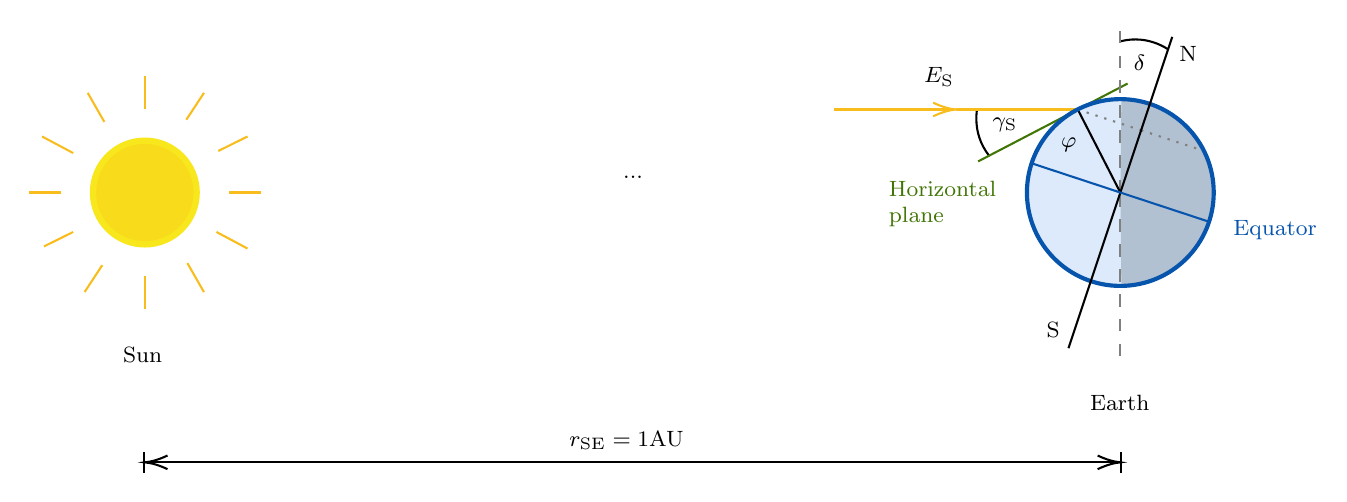
\begin{tikzpicture}[x=0.75pt,y=0.75pt,yscale=-1,xscale=1]
%uncomment if require: \path (0,447); %set diagram left start at 0, and has height of 447

%Shape: Pie [id:dp15034815819494352] 
\draw  [color={rgb, 255:red, 0; green, 0; blue, 0 }  ,draw opacity=0 ][fill={rgb, 255:red, 0; green, 0; blue, 0 }  ,fill opacity=0.45 ] (545.51,179.99) .. controls (570.29,180.26) and (590.33,200.21) .. (590.41,224.85) .. controls (590.49,249.59) and (570.42,269.74) .. (545.5,270.01) -- (545,225) -- cycle ;
%Shape: Circle [id:dp11400902817768599] 
\draw  [color={rgb, 255:red, 7; green, 84; blue, 173 }  ,draw opacity=1 ][fill={rgb, 255:red, 200; green, 222; blue, 248 }  ,fill opacity=0.64 ][line width=0.75]  (500,225) .. controls (500,200.15) and (520.15,180) .. (545,180) .. controls (569.85,180) and (590,200.15) .. (590,225) .. controls (590,249.85) and (569.85,270) .. (545,270) .. controls (520.15,270) and (500,249.85) .. (500,225) -- cycle ;
%Straight Lines [id:da48130102628083926] 
\draw [color={rgb, 255:red, 65; green, 117; blue, 5 }  ,draw opacity=1 ]   (548.5,172.5) -- (524.5,185) ;
%Shape: Arc [id:dp6322515277427461] 
\draw  [draw opacity=0] (481.9,207.42) .. controls (480.77,206.02) and (479.77,204.5) .. (478.91,202.87) .. controls (475.99,197.34) and (475.08,191.17) .. (475.92,184.97) -- (518.5,182) -- cycle ; \draw   (481.9,207.42) .. controls (480.77,206.02) and (479.77,204.5) .. (478.91,202.87) .. controls (475.99,197.34) and (475.08,191.17) .. (475.92,184.97) ;
%Straight Lines [id:da15968904032085707] 
\draw [color={rgb, 255:red, 65; green, 117; blue, 5 }  ,draw opacity=1 ]   (476.5,210) -- (524.5,185) ;
%Shape: Circle [id:dp68849801426956] 
\draw  [color={rgb, 255:red, 248; green, 231; blue, 28 }  ,draw opacity=1 ][fill={rgb, 255:red, 248; green, 220; blue, 28 }  ,fill opacity=1 ][line width=2.25]  (50,225) .. controls (50,211.19) and (61.19,200) .. (75,200) .. controls (88.81,200) and (100,211.19) .. (100,225) .. controls (100,238.81) and (88.81,250) .. (75,250) .. controls (61.19,250) and (50,238.81) .. (50,225) -- cycle ;
%Shape: Arc [id:dp11190386681659015] 
\draw  [draw opacity=0] (544.71,152.26) .. controls (547.24,151.56) and (549.86,151.21) .. (552.55,151.25) .. controls (558.14,151.31) and (563.41,153.04) .. (568.08,156.04) -- (552,196) -- cycle ; \draw   (544.71,152.26) .. controls (547.24,151.56) and (549.86,151.21) .. (552.55,151.25) .. controls (558.14,151.31) and (563.41,153.04) .. (568.08,156.04) ;
%Straight Lines [id:da09161822286264387] 
\draw [color={rgb, 255:red, 128; green, 128; blue, 128 }  ,draw opacity=1 ] [dash pattern={on 4.5pt off 4.5pt}]  (545,303.92) -- (545,225) ;
%Straight Lines [id:da48620147126216584] 
\draw [color={rgb, 255:red, 128; green, 128; blue, 128 }  ,draw opacity=1 ] [dash pattern={on 4.5pt off 4.5pt}]  (545,225) -- (545,146.08) ;
%Straight Lines [id:da2344822206483721] 
\draw [line width=0.75]    (524.5,185) -- (545,225) ;
%Straight Lines [id:da23327222270661996] 
\draw    (77,355) -- (543,355) ;
\draw [shift={(545,355)}, rotate = 180] [color={rgb, 255:red, 0; green, 0; blue, 0 }  ][line width=0.75]    (10.93,-3.29) .. controls (6.95,-1.4) and (3.31,-0.3) .. (0,0) .. controls (3.31,0.3) and (6.95,1.4) .. (10.93,3.29)   ;
\draw [shift={(75,355)}, rotate = 0] [color={rgb, 255:red, 0; green, 0; blue, 0 }  ][line width=0.75]    (10.93,-3.29) .. controls (6.95,-1.4) and (3.31,-0.3) .. (0,0) .. controls (3.31,0.3) and (6.95,1.4) .. (10.93,3.29)   ;
%Straight Lines [id:da6929947931128337] 
\draw [color={rgb, 255:red, 248; green, 189; blue, 28 }  ,draw opacity=1 ]   (407,185) -- (463.75,185) ;
\draw [shift={(465.75,185)}, rotate = 180] [color={rgb, 255:red, 248; green, 189; blue, 28 }  ,draw opacity=1 ][line width=0.75]    (10.93,-3.29) .. controls (6.95,-1.4) and (3.31,-0.3) .. (0,0) .. controls (3.31,0.3) and (6.95,1.4) .. (10.93,3.29)   ;
%Straight Lines [id:da9358361305294991] 
\draw [color={rgb, 255:red, 248; green, 189; blue, 28 }  ,draw opacity=1 ]   (524.5,185) -- (465.75,185) ;
%Straight Lines [id:da7529976931050752] 
\draw    (545.5,350) -- (545.5,360) ;
%Straight Lines [id:da4019381676598568] 
\draw [color={rgb, 255:red, 128; green, 128; blue, 128 }  ,draw opacity=1 ] [dash pattern={on 0.84pt off 2.51pt}]  (555,195) -- (585.5,205) ;
%Straight Lines [id:da051171793746800365] 
\draw [color={rgb, 255:red, 128; green, 128; blue, 128 }  ,draw opacity=1 ] [dash pattern={on 0.84pt off 2.51pt}]  (524.5,185) -- (555,195) ;
%Shape: Circle [id:dp6054942149883367] 
\draw  [color={rgb, 255:red, 7; green, 84; blue, 173 }  ,draw opacity=1 ][fill={rgb, 255:red, 200; green, 222; blue, 248 }  ,fill opacity=0 ][line width=1.5]  (500,225) .. controls (500,200.15) and (520.15,180) .. (545,180) .. controls (569.85,180) and (590,200.15) .. (590,225) .. controls (590,249.85) and (569.85,270) .. (545,270) .. controls (520.15,270) and (500,249.85) .. (500,225) -- cycle ;
%Straight Lines [id:da7513058172554794] 
\draw    (545,225) -- (520,300) ;
%Straight Lines [id:da456675238429898] 
\draw    (570,150) -- (545,225) ;
%Straight Lines [id:da7902385793672442] 
\draw [color={rgb, 255:red, 7; green, 84; blue, 173 }  ,draw opacity=1 ]   (502.5,211) -- (545,225) ;
%Straight Lines [id:da2311496114593583] 
\draw [color={rgb, 255:red, 7; green, 84; blue, 173 }  ,draw opacity=1 ]   (545,225) -- (587.5,239) ;
%Straight Lines [id:da7859324779499595] 
\draw [color={rgb, 255:red, 248; green, 189; blue, 28 }  ,draw opacity=1 ]   (75,169.06) -- (75,184.63) ;
%Straight Lines [id:da6628690922559444] 
\draw [color={rgb, 255:red, 248; green, 189; blue, 28 }  ,draw opacity=1 ]   (130.94,225) -- (115.38,225) ;
%Straight Lines [id:da059104507396427586] 
\draw [color={rgb, 255:red, 248; green, 189; blue, 28 }  ,draw opacity=1 ]   (75,280.94) -- (75,265.38) ;
%Straight Lines [id:da13924610653156622] 
\draw [color={rgb, 255:red, 248; green, 189; blue, 28 }  ,draw opacity=1 ]   (34.63,225) -- (19.06,225) ;
%Straight Lines [id:da6612538806605628] 
\draw [color={rgb, 255:red, 248; green, 189; blue, 28 }  ,draw opacity=1 ]   (109.5,244) -- (124.5,252) ;
%Straight Lines [id:da6313529241657796] 
\draw [color={rgb, 255:red, 248; green, 189; blue, 28 }  ,draw opacity=1 ]   (25.5,198) -- (40.5,206) ;
%Straight Lines [id:da5019670096718076] 
\draw [color={rgb, 255:red, 248; green, 189; blue, 28 }  ,draw opacity=1 ]   (124.5,198) -- (110.38,205) ;
%Straight Lines [id:da9267861672263464] 
\draw [color={rgb, 255:red, 248; green, 189; blue, 28 }  ,draw opacity=1 ]   (40.5,244) -- (26.38,251) ;
%Straight Lines [id:da8979247612603714] 
\draw [color={rgb, 255:red, 248; green, 189; blue, 28 }  ,draw opacity=1 ]   (95,189.94) -- (103.5,177) ;
%Straight Lines [id:da4019503947575047] 
\draw [color={rgb, 255:red, 248; green, 189; blue, 28 }  ,draw opacity=1 ]   (46,272.94) -- (54.5,260) ;
%Straight Lines [id:da27205273028090327] 
\draw [color={rgb, 255:red, 248; green, 189; blue, 28 }  ,draw opacity=1 ]   (95.5,259) -- (103.5,273) ;
%Straight Lines [id:da5079939363345163] 
\draw [color={rgb, 255:red, 248; green, 189; blue, 28 }  ,draw opacity=1 ]   (47.5,177) -- (55.5,191) ;
%Straight Lines [id:da7553342413027122] 
\draw    (74.5,360) -- (74.5,350) ;

% Text Node
\draw (515,197.4) node [anchor=north west][inner sep=0.75pt]  [font=\footnotesize]  {$\varphi $};
% Text Node
\draw (63,298) node [anchor=north west][inner sep=0.75pt]  [font=\footnotesize] [align=left] {Sun};
% Text Node
\draw (529,321) node [anchor=north west][inner sep=0.75pt]  [font=\footnotesize] [align=left] {Earth};
% Text Node
\draw (550,157.4) node [anchor=north west][inner sep=0.75pt]  [font=\footnotesize]  {$\delta $};
% Text Node
\draw (598,237) node [anchor=north west][inner sep=0.75pt]  [font=\footnotesize,color={rgb, 255:red, 7; green, 84; blue, 173 }  ,opacity=1 ] [align=left] {Equator};
% Text Node
\draw (482,187.4) node [anchor=north west][inner sep=0.75pt]  [font=\footnotesize]  {$\gamma _{\mathrm{S}}$};
% Text Node
\draw (432,218) node [anchor=north west][inner sep=0.75pt]  [font=\footnotesize,color={rgb, 255:red, 65; green, 117; blue, 5 }  ,opacity=1 ] [align=left] {Horizontal\\plane};
% Text Node
\draw (449,163.4) node [anchor=north west][inner sep=0.75pt]  [font=\footnotesize]  {$E_{\mathrm{S}}$};
% Text Node
\draw (278,338.4) node [anchor=north west][inner sep=0.75pt]  [font=\footnotesize]  {$r_{\mathrm{SE}} =1\mathrm{AU}$};
% Text Node
\draw (572,153) node [anchor=north west][inner sep=0.75pt]  [font=\footnotesize] [align=left] {N};
% Text Node
\draw (508,286) node [anchor=north west][inner sep=0.75pt]  [font=\footnotesize] [align=left] {S};
% Text Node
\draw (304,215.4) node [anchor=north west][inner sep=0.75pt]  [font=\footnotesize]  {$...$};


\end{tikzpicture}

	\caption{Angular relationship between the Sun and Earth. (Recreated from: \cite{Mertens:2015})}
	\label{fig:tikz_angular_relationship}
\end{figure} 

%
%
%

%% Angular relationships %%

\subsection{Angular relationships}
Before the energy yield of a photovoltaic generator (PVG) can be calculated, it is essential to introduce a few important angles -- of which some were already mentioned in the previous subsection -- and define how they are counted in this thesis.

The local latitude $\varphi$ at the equator is $0^\circ$ and it is counted positive towards the north and negative towards the south, with a range of $\left[-90^\circ \text{, } 90^\circ\right]$. And the local \emph{longitude} $\lambda$ is $0^\circ$ at the reference meridian $\lambda_0$ which passes through the Greenwich Observatory in the United Kingdom. $\lambda$ is counted positive east and negative west of Greenwich, with a range of $\left(-180^\circ \text{, } 180^\circ\right]$ \cite{Appelbaum:1993, Karttunen:2006, Wagner:2018}. For completens it shall be mentioned that the latitude $\varphi$ and the longitude $\lambda$ -- for a given location on Earth -- can be obtained from geographical maps or a global positioning system (GPS) device.

The Sun's declination $\delta$ indicates how far the Earth's axis of rotations -- which runs trough the North and South Poles -- leans towards the Sun at solar noon.\footnote{The definition of the solar noon will be explained in the following paragraphs.} Its range is $\left[-90^\circ \text{, } 90^\circ\right]$, although its maximum values for Earth are $-23,45^\circ$ and $23,45^\circ$. $\delta$ is counted negative if the North Pole leans away from the Sun and positive if it leans towards the Sun (compare to figure \ref{fig:tikz_angular_relationship}) \cite{Appelbaum:1993, Karttunen:2006, Mertens:2015, Wagner:2018}. As per \cite{Wagner:2018}, the following approximation for $\delta$ at a given day of the year, with $N_d$ being the \emph{number of days} since January 1\textsuperscript{st},  $mon$ being the \emph{month} and $d$ being the \emph{day}, is sufficient for photovoltaic applications: 

\begin{center}
	\begin{equation} \label{eq:delta}
		\delta = 23,45^\circ \cdot \sin \left(360^\circ \cdot \frac{284\mathrm{d} + N_d}{365\mathrm{d}}\right) \text{,} 
	\end{equation}
\end{center}

\begin{center}
	\begin{equation} \label{eq:delta}
		N_d = 30,3\mathrm{d} \cdot \left(mon - 1\right) + d \text{.}
	\end{equation}
\end{center}

The altitude $\gamma_{\mathrm{S}}$ and the \emph{azimuth} $\alpha_{\mathrm{S}}$ of the Sun, presented in equations \ref{eq:sin_gamma_s} and \ref{eq:cos_alpha_s}, describe its position in the sky over the course of the day, with $\gamma_{\mathrm{S}}$ taking on values within $\left[0^\circ \text{, } 90^\circ\right]$ and $\alpha_{\mathrm{S}}$ taking on values within $\left(-180^\circ \text{, } 180^\circ \right]$. How these angles are measured -- with the corresponding celstial hemisphere of an observer -- is shown in figure \ref{fig:tikz_gamma_s_alpha_s}. For $\gamma_{\mathrm{S}} = 0^\circ$ the Sun is visible at the horizon and for $\gamma_{\mathrm{S}} = 90^\circ$ it is visible at its zenith. For $\alpha_{\mathrm{S}} = 0^\circ$ the Sun is visible exactly in the south and it takes on positive values towards the west and negative values towards the east \cite{Appelbaum:1993, Karttunen:2006, Mertens:2015, Wagner:2018}.

\begin{center}
	\begin{equation} \label{eq:sin_gamma_s}
		\sin \gamma_{\mathrm{S}} = \sin \varphi \, \sin \delta + \cos \varphi \, \cos \delta \, \cos h_{\mathrm{S}}
	\end{equation}
\end{center}

\begin{center}
	\begin{equation} \label{eq:cos_alpha_s}
		\cos \alpha_{\mathrm{S}} = \frac{\sin \varphi \, \cos \delta \, \cos h_{\mathrm{S}} - \cos \varphi \, \sin \delta}{\cos \gamma_{\mathrm{S}}}
	\end{equation}
\end{center}

\begin{figure}[h!]
	\centering
	

\tikzset{every picture/.style={line width=0.75pt}} %set default line width to 0.75pt        

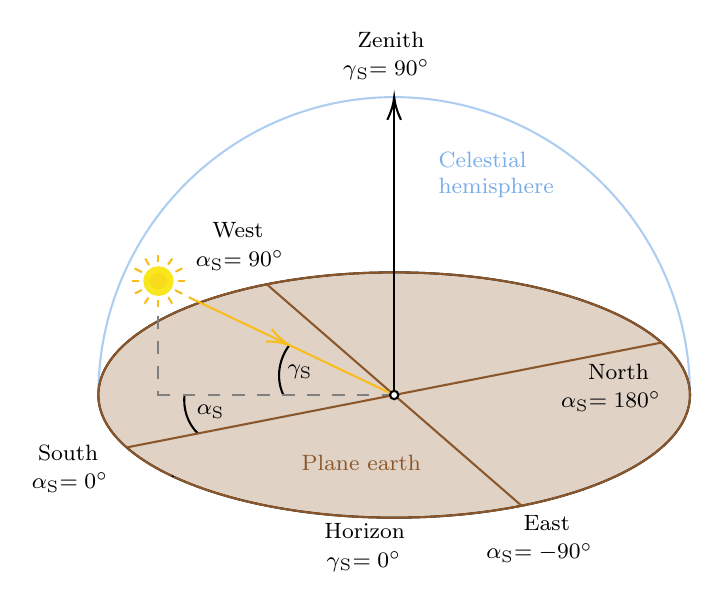
\begin{tikzpicture}[x=0.75pt,y=0.75pt,yscale=-1,xscale=1]
%uncomment if require: \path (0,445); %set diagram left start at 0, and has height of 445






%Shape: Ellipse [id:dp10248886204350427] 
\draw  [color={rgb, 255:red, 0; green, 0; blue, 0 }  ,draw opacity=1 ][fill={rgb, 255:red, 139; green, 87; blue, 42 }  ,fill opacity=0.27 ] (120.55,216.48) .. controls (120.55,183.84) and (184.36,157.39) .. (263.08,157.39) .. controls (341.79,157.39) and (405.61,183.84) .. (405.61,216.48) .. controls (405.61,249.12) and (341.79,275.58) .. (263.08,275.58) .. controls (184.36,275.58) and (120.55,249.12) .. (120.55,216.48) -- cycle ;
%Shape: Arc [id:dp9824695676563142] 
\draw  [draw opacity=0] (120.55,216.48) .. controls (120.55,216.48) and (120.55,216.48) .. (120.55,216.48) .. controls (120.55,137.22) and (184.36,72.96) .. (263.08,72.96) .. controls (341.79,72.96) and (405.61,137.22) .. (405.61,216.48) -- (263.08,216.48) -- cycle ; \draw  [color={rgb, 255:red, 74; green, 144; blue, 226 }  ,draw opacity=0.45 ] (120.55,216.48) .. controls (120.55,216.48) and (120.55,216.48) .. (120.55,216.48) .. controls (120.55,137.22) and (184.36,72.96) .. (263.08,72.96) .. controls (341.79,72.96) and (405.61,137.22) .. (405.61,216.48) ;
%Shape: Ellipse [id:dp6726138734461271] 
\draw  [color={rgb, 255:red, 248; green, 231; blue, 28 }  ,draw opacity=1 ][fill={rgb, 255:red, 248; green, 220; blue, 28 }  ,fill opacity=1 ][line width=2.25]  (143.71,161.61) .. controls (143.71,158.48) and (146.3,155.95) .. (149.5,155.95) .. controls (152.7,155.95) and (155.3,158.48) .. (155.3,161.61) .. controls (155.3,164.73) and (152.7,167.27) .. (149.5,167.27) .. controls (146.3,167.27) and (143.71,164.73) .. (143.71,161.61) -- cycle ;
%Straight Lines [id:da22837958638990763] 
\draw [color={rgb, 255:red, 248; green, 189; blue, 28 }  ,draw opacity=1 ]   (149.5,148.94) -- (149.5,152.47) ;
%Straight Lines [id:da36410436567305116] 
\draw [color={rgb, 255:red, 248; green, 189; blue, 28 }  ,draw opacity=1 ]   (162.47,161.61) -- (158.86,161.61) ;
%Straight Lines [id:da7784535438011968] 
\draw [color={rgb, 255:red, 248; green, 189; blue, 28 }  ,draw opacity=1 ]   (149.5,174.27) -- (149.5,170.75) ;
%Straight Lines [id:da02148874103533327] 
\draw [color={rgb, 255:red, 248; green, 189; blue, 28 }  ,draw opacity=1 ]   (140.14,161.61) -- (136.53,161.61) ;
%Straight Lines [id:da5806655094182651] 
\draw [color={rgb, 255:red, 248; green, 189; blue, 28 }  ,draw opacity=1 ]   (157.5,165.91) -- (160.98,167.72) ;
%Straight Lines [id:da9042107417993022] 
\draw [color={rgb, 255:red, 248; green, 189; blue, 28 }  ,draw opacity=1 ]   (138.03,155.49) -- (141.5,157.31) ;
%Straight Lines [id:da8739850131703888] 
\draw [color={rgb, 255:red, 248; green, 189; blue, 28 }  ,draw opacity=1 ]   (160.98,155.49) -- (157.7,157.08) ;
%Straight Lines [id:da9973855947966144] 
\draw [color={rgb, 255:red, 248; green, 189; blue, 28 }  ,draw opacity=1 ]   (141.5,165.91) -- (138.23,167.49) ;
%Straight Lines [id:da23606504338204548] 
\draw [color={rgb, 255:red, 248; green, 189; blue, 28 }  ,draw opacity=1 ]   (154.14,153.67) -- (156.11,150.74) ;
%Straight Lines [id:da06728456263139648] 
\draw [color={rgb, 255:red, 248; green, 189; blue, 28 }  ,draw opacity=1 ]   (142.78,172.46) -- (144.75,169.53) ;
%Straight Lines [id:da5070173352082208] 
\draw [color={rgb, 255:red, 248; green, 189; blue, 28 }  ,draw opacity=1 ]   (154.26,169.3) -- (156.11,172.47) ;
%Straight Lines [id:da536701929565258] 
\draw [color={rgb, 255:red, 248; green, 189; blue, 28 }  ,draw opacity=1 ]   (143.13,150.74) -- (144.98,153.91) ;
%Straight Lines [id:da1832197332832679] 
\draw [color={rgb, 255:red, 139; green, 87; blue, 42 }  ,draw opacity=1 ]   (324.28,269.67) -- (263.08,216.48) ;
%Straight Lines [id:da35722852927602045] 
\draw [color={rgb, 255:red, 139; green, 87; blue, 42 }  ,draw opacity=1 ]   (263.08,216.48) -- (201.88,163.3) ;
%Shape: Arc [id:dp6576066040432391] 
\draw  [draw opacity=0] (168.58,235.07) .. controls (163.53,230.23) and (161.29,223.2) .. (162.06,216.13) -- (185.16,216.91) -- cycle ; \draw   (168.58,235.07) .. controls (163.53,230.23) and (161.29,223.2) .. (162.06,216.13) ;
%Shape: Arc [id:dp8644885498360859] 
\draw  [draw opacity=0] (209.82,216.7) .. controls (206.04,209.04) and (207.21,199.65) .. (212.57,192.43) -- (231.46,205.17) -- cycle ; \draw   (209.82,216.7) .. controls (206.04,209.04) and (207.21,199.65) .. (212.57,192.43) ;
%Straight Lines [id:da40176543382530383] 
\draw [color={rgb, 255:red, 248; green, 189; blue, 28 }  ,draw opacity=1 ]   (263.08,216.48) -- (212.58,192.42) ;
%Straight Lines [id:da43066607290523007] 
\draw [color={rgb, 255:red, 128; green, 128; blue, 128 }  ,draw opacity=1 ] [dash pattern={on 4.5pt off 4.5pt}]  (149.15,216.48) -- (263.08,216.48) ;
%Straight Lines [id:da9460200323685761] 
\draw [color={rgb, 255:red, 139; green, 87; blue, 42 }  ,draw opacity=1 ]   (133.86,241.81) -- (263.08,216.48) ;
%Straight Lines [id:da12611331746579268] 
\draw [color={rgb, 255:red, 139; green, 87; blue, 42 }  ,draw opacity=1 ]   (263.08,216.48) -- (392.3,191.15) ;
%Shape: Arc [id:dp7682340536128898] 
\draw  [draw opacity=0] (155.96,255.47) .. controls (133.92,245.06) and (120.55,231.42) .. (120.55,216.48) .. controls (120.55,183.84) and (184.36,157.39) .. (263.08,157.39) .. controls (341.79,157.39) and (405.61,183.84) .. (405.61,216.48) .. controls (405.61,249.12) and (341.79,275.58) .. (263.08,275.58) .. controls (220.87,275.58) and (182.95,267.97) .. (156.85,255.88) -- (263.08,216.48) -- cycle ; \draw  [color={rgb, 255:red, 139; green, 87; blue, 42 }  ,draw opacity=1 ] (155.96,255.47) .. controls (133.92,245.06) and (120.55,231.42) .. (120.55,216.48) .. controls (120.55,183.84) and (184.36,157.39) .. (263.08,157.39) .. controls (341.79,157.39) and (405.61,183.84) .. (405.61,216.48) .. controls (405.61,249.12) and (341.79,275.58) .. (263.08,275.58) .. controls (220.87,275.58) and (182.95,267.97) .. (156.85,255.88) ;
%Straight Lines [id:da15722411504245715] 
\draw [color={rgb, 255:red, 128; green, 128; blue, 128 }  ,draw opacity=1 ] [dash pattern={on 4.5pt off 4.5pt}]  (149.5,178.56) -- (149.5,216.93) ;
%Straight Lines [id:da003502427569964439] 
\draw [color={rgb, 255:red, 248; green, 189; blue, 28 }  ,draw opacity=1 ]   (210.77,191.57) -- (164.08,169.36) ;
\draw [shift={(212.57,192.43)}, rotate = 205.44] [color={rgb, 255:red, 248; green, 189; blue, 28 }  ,draw opacity=1 ][line width=0.75]    (10.93,-3.29) .. controls (6.95,-1.4) and (3.31,-0.3) .. (0,0) .. controls (3.31,0.3) and (6.95,1.4) .. (10.93,3.29)   ;
%Straight Lines [id:da8840339574734517] 
\draw    (263.08,216.48) -- (263.08,74.96) ;
\draw [shift={(263.08,72.96)}, rotate = 450] [color={rgb, 255:red, 0; green, 0; blue, 0 }  ][line width=0.75]    (10.93,-3.29) .. controls (6.95,-1.4) and (3.31,-0.3) .. (0,0) .. controls (3.31,0.3) and (6.95,1.4) .. (10.93,3.29)   ;
%Shape: Circle [id:dp5710959149747352] 
\draw  [fill={rgb, 255:red, 255; green, 255; blue, 255 }  ,fill opacity=1 ] (261.08,216.48) .. controls (261.08,215.38) and (261.97,214.48) .. (263.08,214.48) .. controls (264.18,214.48) and (265.08,215.38) .. (265.08,216.48) .. controls (265.08,217.59) and (264.18,218.48) .. (263.08,218.48) .. controls (261.97,218.48) and (261.08,217.59) .. (261.08,216.48) -- cycle ;

% Text Node
\draw (210.29,200.68) node [anchor=north west][inner sep=0.75pt]  [font=\footnotesize]  {$\gamma _{\mathrm{S}}$};
% Text Node
\draw (166.49,219.8) node [anchor=north west][inner sep=0.75pt]  [font=\footnotesize]  {$\alpha _{\mathrm{S}}$};
% Text Node
\draw (217,244) node [anchor=north west][inner sep=0.75pt]  [font=\footnotesize,color={rgb, 255:red, 139; green, 87; blue, 42 }  ,opacity=1 ] [align=left] {Plane earth};
% Text Node
\draw (87,252.4) node [anchor=north west][inner sep=0.75pt]  [font=\footnotesize]  {$\textcolor[rgb]{0,0,0}{\alpha }\textcolor[rgb]{0,0,0}{_{\mathrm{S}}}\textcolor[rgb]{0,0,0}{=0}\textcolor[rgb]{0,0,0}{^{\circ }}$};
% Text Node
\draw (90,239) node [anchor=north west][inner sep=0.75pt]  [font=\footnotesize] [align=left] {South};
% Text Node
\draw (324,273) node [anchor=north west][inner sep=0.75pt]  [font=\footnotesize] [align=left] {East};
% Text Node
\draw (306,286.4) node [anchor=north west][inner sep=0.75pt]  [font=\footnotesize]  {$\textcolor[rgb]{0,0,0}{\alpha }\textcolor[rgb]{0,0,0}{_{\mathrm{S}}}\textcolor[rgb]{0,0,0}{=-90}\textcolor[rgb]{0,0,0}{^{\circ }}$};
% Text Node
\draw (244,40) node [anchor=north west][inner sep=0.75pt]  [font=\footnotesize] [align=left] {Zenith};
% Text Node
\draw (237,53.4) node [anchor=north west][inner sep=0.75pt]  [font=\footnotesize]  {$\textcolor[rgb]{0,0,0}{\gamma }\textcolor[rgb]{0,0,0}{_{\mathrm{S}}}\textcolor[rgb]{0,0,0}{=90}\textcolor[rgb]{0,0,0}{^{\circ }}$};
% Text Node
\draw (174,132) node [anchor=north west][inner sep=0.75pt]  [font=\footnotesize] [align=left] {West};
% Text Node
\draw (166,145.4) node [anchor=north west][inner sep=0.75pt]  [font=\footnotesize]  {$\textcolor[rgb]{0,0,0}{\alpha }\textcolor[rgb]{0,0,0}{_{\mathrm{S}}}\textcolor[rgb]{0,0,0}{=90}\textcolor[rgb]{0,0,0}{^{\circ }}$};
% Text Node
\draw (342,213.4) node [anchor=north west][inner sep=0.75pt]  [font=\footnotesize]  {$\textcolor[rgb]{0,0,0}{\alpha }\textcolor[rgb]{0,0,0}{_{\mathrm{S}}}\textcolor[rgb]{0,0,0}{=180}\textcolor[rgb]{0,0,0}{^{\circ }}$};
% Text Node
\draw (355,200) node [anchor=north west][inner sep=0.75pt]  [font=\footnotesize] [align=left] {North};
% Text Node
\draw (229,290.4) node [anchor=north west][inner sep=0.75pt]  [font=\footnotesize]  {$\textcolor[rgb]{0,0,0}{\gamma }\textcolor[rgb]{0,0,0}{_{\mathrm{S}}}\textcolor[rgb]{0,0,0}{=0}\textcolor[rgb]{0,0,0}{^{\circ }}$};
% Text Node
\draw (228,277) node [anchor=north west][inner sep=0.75pt]  [font=\footnotesize] [align=left] {Horizon};
% Text Node
\draw (283,98) node [anchor=north west][inner sep=0.75pt]  [font=\footnotesize,color={rgb, 255:red, 74; green, 144; blue, 226 }  ,opacity=0.74 ] [align=left] {Celestial\\hemisphere};


\end{tikzpicture}

	\caption{From the view of an observer on Earth, the Sun reaches its greates altitude at the solar noon ($h_{\mathrm{S}} = 0^\circ$) in the south. In this figure the Sun already passed the solar noon. (Recreated from: \cite{Mertens:2015})}
	\label{fig:tikz_gamma_s_alpha_s}
\end{figure}

It must be noted that $\gamma_{\mathrm{S}}$ and $\alpha_{\mathrm{S}}$ change over the course of the day. By analyzing equations \ref{eq:sin_gamma_s} and \ref{eq:cos_alpha_s}, while taking into account that $\varphi$ does not change because the self-sufficient BVCR is stationary, and that, in this thesis, $\delta$ is modeled with a constant value throughout the day -- altough it takes on different values for each day of the year -- it must be the variable $h_{\mathrm{S}}$ that is responsible for these changes. It is called the \emph{solar hour angle} and its value is $0^\circ$ when the Sun reaches its greatest daily altitude $\gamma_{\mathrm{S}}$ at solar noon. This happens for either $\alpha_{\mathrm{S}} = 0^\circ$, $\alpha_{\mathrm{S}} = 180^\circ$ or for $\gamma_{\mathrm{S}} = 90^\circ$ where $\alpha_{\mathrm{S}}$ is undefined. $h_{\mathrm{S}}$ is counted negative before the solar noon and positive after the solar noon, with a range of $\left(-180^\circ \text{, } 180^\circ\right]$. \cite{Appelbaum:1993, Karttunen:2006, Mertens:2015, Wagner:2018}.  

For a given \emph{solar time}\footnote{In the most cases the solar time $t_\mathrm{S}$ differs from the local time on a wrist watch. For $t_\mathrm{S} = 12\mathrm{h}$ (noon) the Sun is either exaclty in the south or in the north, whereas the Sun might not be exactly in the south, nor in the north, for the \emph{local time} $t_\mathrm{local} = 12\mathrm{h}$, on a wrist watch -- no matter how accurate it is set to the local time. More information can be obtained from \cite{Mertens:2015, Wagner:2018}.} $t_\mathrm{S}$, the hour angle $h_\mathrm{S}$ can be determined as shown in equation \ref{eq:solar_hour_angle}. The factor $\frac{15^\circ}{1\mathrm{h}}$ comes about because the Earth rotates $360^\circ$ within $24\mathrm{h}$, thus the range of the solar time $t_\mathrm{S}$ can be derived to $\left[0\mathrm{h} \text{, } 24\mathrm{h}\right)$. And the hour angle for the \emph{solar sunrise time} $t_\mathrm{S,r}$ and the \emph{solar sunset time} $t_\mathrm{S,s}$ can be calculated with the equations \ref{eq:h_sunrise} and \ref{eq:h_sunset} \cite{Appelbaum:1993, Karttunen:2006, Mertens:2015, Wagner:2018}.

\begin{center}
	\begin{equation} \label{eq:solar_hour_angle}
		h_\mathrm{S} = \left(t_\mathrm{S} - 12\mathrm{h} \right) \cdot \frac{15^\circ}{1\mathrm{h}}
	\end{equation}
\end{center}

\begin{center}
	\begin{equation} \label{eq:h_sunrise}
		h_\mathrm{S,r} = - \arccos \left( -\tan \delta \tan \, \varphi \right) \text{,} \quad \text{for } \left|\varphi\right| < 90^\circ - \left|\delta\right|
	\end{equation}
\end{center}

\begin{center}
	\begin{equation} \label{eq:h_sunset}
		h_\mathrm{S,s} = \arccos \left( -\tan \delta \, \tan \varphi \right) \text{,} \quad \text{for } \left|\varphi\right| < 90^\circ - \left|\delta\right|
	\end{equation}
\end{center}

In \cite{Appelbaum:1993} a few special cases for equations \ref{eq:h_sunrise} and \ref{eq:h_sunset} are mentioned which, might be of interest when choosing mission locations for the self-sufficient BVCR:

%\vspace{2mm}
\[ \tan \delta \, \tan \varphi \,
  \begin{cases}
    > 1       	& \quad \text{polar night, if } \varphi < -90^\circ + \delta \text{ or } \varphi > 90^\circ + \delta \text{,} \\
    = \pm 1  		& \quad \text{the Sun is only visible at the horizon for an instant,} \\
    < -1		& \quad \text{polar day, if } \varphi < -90^\circ - \delta \text{ or } \varphi > 90^\circ - \delta \text{.}
  \end{cases}
\]
%\vspace{2mm}

The solar time $t_\mathrm{S}$ can furthermore be calculated from $t_\mathrm{UTC}$, which is the \emph{Coordinated Universal Time} (UTC), using the equation \ref{eq:solar_time}, where $\lambda_0 = 0^\circ$ is the reference meridian for which $t_\mathrm{UTC}$ applies and $Z_{\mathrm{h}}$ is the \emph{equation of time} which serves as a correction factor. More information about these equations is provided by \cite{Karttunen:2006, Wagner:2018}.

\begin{center}
	\begin{equation} \label{eq:solar_time}
		t_\mathrm{S} = t_\mathrm{UTC} + Z_{\mathrm{h}} + \left(\lambda - \lambda_{\mathrm{0}}\right) \cdot \frac{1\mathrm{h}}{15\degree}
	\end{equation}
\end{center}

\begin{center}
	\begin{equation} \label{eq:time_equation}
		Z_{\mathrm{h}} = 0,123\mathrm{h} \cdot \cos \left(360^\circ \cdot \frac{88\mathrm{d} + N_d}{365\mathrm{d}}\right) - 0,167\mathrm{h} \cdot \sin \left(720^\circ \cdot \frac{10\mathrm{d} + N_d}{365\mathrm{d}}\right) 
	\end{equation}
\end{center}

%
%
%

%% Solar irradiation on Earth's surface %%

\subsection{Solar irradiation on Earth's surface} \label{sec:solar_irradiation_on_earths_surface}
Compared to equation \ref{eq:e_sun}, determining the Sun's irradiance arriving on the ground is rather complex.\footnote{In \cite{Appelbaum:1989, Appelbaum:1992} this topic is investigated for the planet Mars.} Precise calculations depend on many different factors such as the changing angular relationship between the Earth and the Sun throughout the year, the composition of the Earth's atmosphere -- which changes the Sun's spectrum due to absorbtion and scattering effects -- and many more \cite{Appelbaum:1993, Mertens:2015, Wagner:2018}. 

\begin{figure}[h!]
	\centering
  	\includegraphics[width = 0.96\textwidth]{solar_maps/austria/austria_ghi}
  	\caption{Solar resource map of the long term average global horizontal irradiation of Austria. (Image credit: \emph{www.solargis.com} and \emph{www.globalsolaratlas.info})}
	\label{fig:ghi_austria}
\end{figure}

With solar resource maps however, this problem can be circumvented. They are based on satellite and atmospheric solar irradiance models and meteorological data, that were designed and collected over several years. By using these maps, the compromise is made, that the following calculations and estimates are performed with average irradiance values instead of exact ones.\footnote{If exact irradiance values are known, the equations presented in the following subsections can provide more accurate estimates.} Figures \ref{fig:ghi_austria} and \ref{fig:dni_austria} provided by \cite{SolargisMaps:2020, GlobalSolarAtlas:2020} show the solar resource maps of the long term average global horizontal and direct normal irradiation, from 1994 until 2018, of Austria. The scale below the maps shows daily and annual total irradiation in $\mathrm{kWh}/\mathrm{m}^2$ \cite{MeteorologicalModeling:2020, SolarRadiationModeling:2020, SolargisData:2020}. 

\begin{figure}[h!]
	\centering
  	\includegraphics[width = 0.96\textwidth]{solar_maps/austria/austria_dni}
	\caption{Solar resource map of the long term average direct normal irradiation of Austria. (Image credit: \emph{www.solargis.com} and \emph{www.globalsolaratlas.info})}
	\label{fig:dni_austria}
\end{figure}

It can be clearly seen that the values for both the global horizontal and the direct normal irradiation tend to be higher in the south and lower in the north of Austria. This can be partly explained by a greater latitude $\varphi$ which results in a lower altitude of the Sun $\gamma_{\mathrm{S}}$ during the winter months on the northern hemisphere ($\delta < 0$). Because of this, the Sun's incoming rays need to penetrate a thicker atmopshere and it is visible above the horizon for a shorter period of time over the course of the day. For locations in the south, such as the region around Klagenfurt, daily global horizontal irradiation totals of up to $3,50\mathrm{kWh}/\mathrm{m}^2$ and direct normal irradiation totals of up to $3,55\mathrm{kWh}/\mathrm{m}^2$ and higher can be expected, whereas loactions in the north, for example Linz, only reach daily global horizontal irradiation totals of around $3,25\mathrm{kWh}/\mathrm{m}^2$ and daily direct normal irradiation totals of around $2,9\mathrm{kWh}/\mathrm{m}^2$. Another notable feature are valleys bordered by mountains in the south. In these valleys, and on the bounding north-facing mountain slopes, the daily global horizontal irradiation total drops to less than $2,5\mathrm{kWh}/\mathrm{m}^2$ and the daily direct normal irradiation total drops even further down to around $1,5\mathrm{kWh}/\mathrm{m}^2$. Examples for such valleys can be located all across the Alps and they highlight, that locations, with geographical features that block the direct path of the sunlight, should be discarded as installation sites for a PVG \cite{Karttunen:2006, Mertens:2015, Wagner:2018}.

Using solar resource maps, the \emph{global horizontal irradiance} (GHI) $E_{\mathrm{GHI}}$ and the \emph{direct normal irradiance} (DNI) $E_{\mathrm{DNI}}$ -- at a given location on Earth -- can be determined by either, dividing the values of the global horizontal and the direct normal irradiation by $24\mathrm{h}$, or by $365\mathrm{d} \cdot 24\mathrm{h}$ -- depending on the used scale. Therefore the unit of the GHI and the DNI is $\mathrm{W}/\mathrm{m}^2$ \cite{Mertens:2015, SolargisData:2020}.

As mentioned in \cite{Mertens:2015, SolarRadiationModeling:2020} and shown in equation \ref{eq:e_ghi}, the GHI results from the \emph{direct horizontal irradiance} (DHI) $E_{\mathrm{DHI}}$ and the \emph{diffuse horizontal irradiance} (DIFH) $E_{\mathrm{DIFH}}$. The latter is caused by the scattering of sunlight by Earth's atmosphere.

\begin{center}
	\begin{equation} \label{eq:e_ghi}
		E_{\mathrm{GHI}} = E_{\mathrm{DHI}} + E_{\mathrm{DIFH}}
	\end{equation}
\end{center}

In comparison to the GHI -- which applies to a horizontal surface -- the DNI applies to a flat surface element perpendicular to the incoming Sun rays, and it only consideres the direct irradiance \cite{Mertens:2015, SolarRadiationModeling:2020}. With simple trigonometry as shown in \cite{Mertens:2015}, the relationship between $E_{\mathrm{DNI}}$ and $E_{\mathrm{DHI}}$ can be written as:

\begin{center}
	\begin{equation} \label{eq:e_dni}
		E_{\mathrm{DNI}} = E_{\mathrm{DHI}} \, \frac{1}{\sin \gamma_{\mathrm{S}}} \text{.}
	\end{equation}
\end{center}

Since solar resource maps are used in this thesis to obtain the irradiance values presented in the equations \ref{eq:e_ghi} and \ref{eq:e_dni}, more global horizontal and direct normal irradiation solar resource maps of Israel, Oman and Chile as well as for Europe and the World, can be found in appeendix \ref{ap:solar_resource_maps}. More precise solar resource maps for daily and monthly global horizontal and direct normal irradiation are provided by \cite{Union:2020}.

%
%
%

%% Photovoltaic energy yield %%

\subsection{Photovoltaic energy yield} \label{sec:energy_yield}
As already mentioned in subsection \ref{sec:solar_irradiation_on_earths_surface} the decisive factors to determine the irradiance at a given location on the Earth's surface, are the GHI and the DNI. Based on these, the three-component model as described in \cite{Appelbaum:1993, Mertens:2015}, can be used to calculate the \emph{total irradiance} $E_{\mathrm{GEN}}$ received by an inclined PVG. In this thesis, the angle of inclination, with respect to the ground, is $\beta$. An example for such an inclined PVG is shown in figure \ref{fig:tikz_three_component_model}.
\begin{figure}[h!]
	\centering
	

\tikzset{every picture/.style={line width=0.75pt}} %set default line width to 0.75pt        

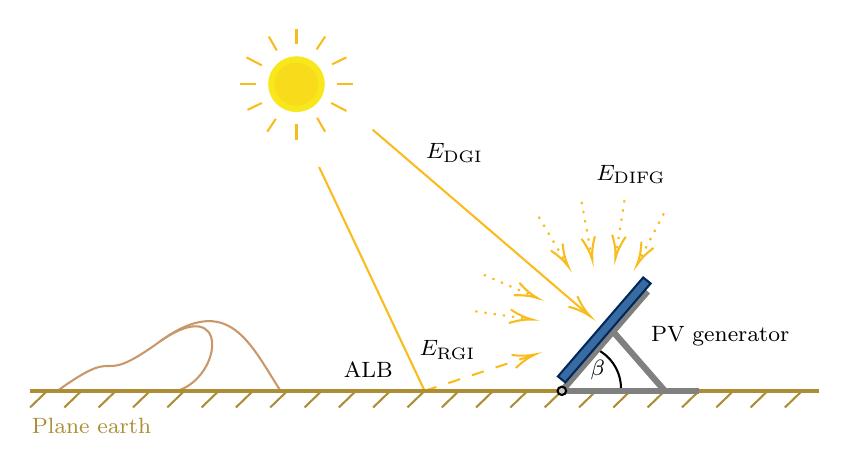
\begin{tikzpicture}[x=0.75pt,y=0.75pt,yscale=-1,xscale=1]
%uncomment if require: \path (0,468); %set diagram left start at 0, and has height of 468

%Straight Lines [id:da7639591375517361] 
\draw [color={rgb, 255:red, 248; green, 189; blue, 28 }  ,draw opacity=1 ]   (249.06,186.64) -- (299.9,294.48) ;
%Shape: Ellipse [id:dp07145193932966887] 
\draw  [color={rgb, 255:red, 248; green, 231; blue, 28 }  ,draw opacity=1 ][fill={rgb, 255:red, 248; green, 220; blue, 28 }  ,fill opacity=1 ][line width=2.25]  (226.02,146.71) .. controls (226.02,140.12) and (231.45,134.77) .. (238.15,134.77) .. controls (244.85,134.77) and (250.29,140.12) .. (250.29,146.71) .. controls (250.29,153.31) and (244.85,158.65) .. (238.15,158.65) .. controls (231.45,158.65) and (226.02,153.31) .. (226.02,146.71) -- cycle ;
%Curve Lines [id:da4839167804983171] 
\draw [color={rgb, 255:red, 202; green, 151; blue, 106 }  ,draw opacity=1 ]   (172.61,270.51) .. controls (206.08,247.35) and (202.78,287.29) .. (180.87,294.48) ;
%Curve Lines [id:da9367845814708875] 
\draw [color={rgb, 255:red, 202; green, 151; blue, 106 }  ,draw opacity=1 ]   (123.01,294.48) .. controls (156.08,270.51) and (139.55,294.48) .. (172.61,270.51) .. controls (205.67,246.55) and (216,272.11) .. (230.47,294.48) ;
%Straight Lines [id:da20208524763476388] 
\draw [color={rgb, 255:red, 248; green, 189; blue, 28 }  ,draw opacity=1 ] [dash pattern={on 4.5pt off 4.5pt}]  (299.9,294.48) -- (351.31,277.53) ;
\draw [shift={(353.21,276.9)}, rotate = 521.76] [color={rgb, 255:red, 248; green, 189; blue, 28 }  ,draw opacity=1 ][line width=0.75]    (10.93,-3.29) .. controls (6.95,-1.4) and (3.31,-0.3) .. (0,0) .. controls (3.31,0.3) and (6.95,1.4) .. (10.93,3.29)   ;
%Curve Lines [id:da8387867434601526] 
\draw    (382.96,274.51) .. controls (387.92,276.9) and (394.53,283.29) .. (394.53,293.68) ;
%Straight Lines [id:da056555134551903974] 
\draw [color={rgb, 255:red, 173; green, 142; blue, 55 }  ,draw opacity=1 ][fill={rgb, 255:red, 139; green, 87; blue, 42 }  ,fill opacity=1 ][line width=1.5]    (109.79,294.48) -- (490,294.48) ;
%Straight Lines [id:da48348316265398994] 
\draw [color={rgb, 255:red, 173; green, 142; blue, 55 }  ,draw opacity=1 ]   (134.59,294.48) -- (126.32,302.47) ;
%Straight Lines [id:da4565238298434817] 
\draw [color={rgb, 255:red, 173; green, 142; blue, 55 }  ,draw opacity=1 ]   (151.12,294.48) -- (142.85,302.47) ;
%Straight Lines [id:da7555358341240341] 
\draw [color={rgb, 255:red, 173; green, 142; blue, 55 }  ,draw opacity=1 ]   (167.65,294.48) -- (159.38,302.47) ;
%Straight Lines [id:da10247707612378121] 
\draw [color={rgb, 255:red, 173; green, 142; blue, 55 }  ,draw opacity=1 ]   (184.18,294.48) -- (175.91,302.47) ;
%Straight Lines [id:da22505664528789526] 
\draw [color={rgb, 255:red, 173; green, 142; blue, 55 }  ,draw opacity=1 ]   (200.71,294.48) -- (192.44,302.47) ;
%Straight Lines [id:da39883233893640213] 
\draw [color={rgb, 255:red, 173; green, 142; blue, 55 }  ,draw opacity=1 ]   (217.24,294.48) -- (208.98,302.47) ;
%Straight Lines [id:da9317267044471207] 
\draw [color={rgb, 255:red, 173; green, 142; blue, 55 }  ,draw opacity=1 ]   (233.77,294.48) -- (225.51,302.47) ;
%Straight Lines [id:da5689034971431022] 
\draw [color={rgb, 255:red, 173; green, 142; blue, 55 }  ,draw opacity=1 ]   (118.06,294.48) -- (109.79,302.47) ;
%Straight Lines [id:da6794614658982192] 
\draw [color={rgb, 255:red, 173; green, 142; blue, 55 }  ,draw opacity=1 ]   (250.3,294.48) -- (242.04,302.47) ;
%Straight Lines [id:da16884333894084147] 
\draw [color={rgb, 255:red, 173; green, 142; blue, 55 }  ,draw opacity=1 ]   (266.83,294.48) -- (258.57,302.47) ;
%Straight Lines [id:da5852948402158396] 
\draw [color={rgb, 255:red, 173; green, 142; blue, 55 }  ,draw opacity=1 ]   (283.36,294.48) -- (275.1,302.47) ;
%Straight Lines [id:da5569944189270981] 
\draw [color={rgb, 255:red, 173; green, 142; blue, 55 }  ,draw opacity=1 ]   (299.9,294.48) -- (291.63,302.47) ;
%Straight Lines [id:da07636127130608306] 
\draw [color={rgb, 255:red, 173; green, 142; blue, 55 }  ,draw opacity=1 ]   (316.43,294.48) -- (308.16,302.47) ;
%Straight Lines [id:da7270434905185723] 
\draw [color={rgb, 255:red, 173; green, 142; blue, 55 }  ,draw opacity=1 ]   (332.96,294.48) -- (324.69,302.47) ;
%Straight Lines [id:da5998901663023846] 
\draw [color={rgb, 255:red, 173; green, 142; blue, 55 }  ,draw opacity=1 ]   (349.49,294.48) -- (341.22,302.47) ;
%Straight Lines [id:da2586618910795322] 
\draw [color={rgb, 255:red, 173; green, 142; blue, 55 }  ,draw opacity=1 ]   (366.02,294.48) -- (357.75,302.47) ;
%Straight Lines [id:da2230405823513728] 
\draw [color={rgb, 255:red, 173; green, 142; blue, 55 }  ,draw opacity=1 ]   (382.55,294.48) -- (374.28,302.47) ;
%Straight Lines [id:da33268357962040995] 
\draw [color={rgb, 255:red, 173; green, 142; blue, 55 }  ,draw opacity=1 ]   (399.08,294.48) -- (390.81,302.47) ;
%Straight Lines [id:da9040529515577587] 
\draw [color={rgb, 255:red, 173; green, 142; blue, 55 }  ,draw opacity=1 ]   (415.61,294.48) -- (407.35,302.47) ;
%Straight Lines [id:da9864302443455792] 
\draw [color={rgb, 255:red, 173; green, 142; blue, 55 }  ,draw opacity=1 ]   (432.14,294.48) -- (423.88,302.47) ;
%Straight Lines [id:da5062470043832821] 
\draw [color={rgb, 255:red, 173; green, 142; blue, 55 }  ,draw opacity=1 ]   (448.67,294.48) -- (440.41,302.47) ;
%Straight Lines [id:da3838353864046502] 
\draw [color={rgb, 255:red, 173; green, 142; blue, 55 }  ,draw opacity=1 ]   (465.2,294.48) -- (456.94,302.47) ;
%Straight Lines [id:da7629428788396968] 
\draw [color={rgb, 255:red, 173; green, 142; blue, 55 }  ,draw opacity=1 ]   (481.73,294.48) -- (473.47,302.47) ;
%Straight Lines [id:da014514371361068923] 
\draw [color={rgb, 255:red, 128; green, 128; blue, 128 }  ,draw opacity=1 ][line width=2.25]    (407.35,246.55) -- (366.02,294.48) ;
%Straight Lines [id:da49954840219882635] 
\draw [color={rgb, 255:red, 128; green, 128; blue, 128 }  ,draw opacity=1 ][line width=2.25]    (432.14,294.48) -- (366.02,294.48) ;
%Straight Lines [id:da9965546684463125] 
\draw [color={rgb, 255:red, 128; green, 128; blue, 128 }  ,draw opacity=1 ][line width=2.25]    (391.23,266.52) -- (415.61,294.48) ;
%Straight Lines [id:da9786945806038319] 
\draw [color={rgb, 255:red, 248; green, 189; blue, 28 }  ,draw opacity=1 ] [dash pattern={on 0.84pt off 2.51pt}]  (415.2,209.01) -- (403.11,232) ;
\draw [shift={(402.18,233.77)}, rotate = 297.73] [color={rgb, 255:red, 248; green, 189; blue, 28 }  ,draw opacity=1 ][line width=0.75]    (10.93,-3.29) .. controls (6.95,-1.4) and (3.31,-0.3) .. (0,0) .. controls (3.31,0.3) and (6.95,1.4) .. (10.93,3.29)   ;
%Straight Lines [id:da4673310913126938] 
\draw [color={rgb, 255:red, 248; green, 189; blue, 28 }  ,draw opacity=1 ] [dash pattern={on 0.84pt off 2.51pt}]  (324.28,256.14) -- (349.78,259.84) ;
\draw [shift={(351.76,260.13)}, rotate = 188.27] [color={rgb, 255:red, 248; green, 189; blue, 28 }  ,draw opacity=1 ][line width=0.75]    (10.93,-3.29) .. controls (6.95,-1.4) and (3.31,-0.3) .. (0,0) .. controls (3.31,0.3) and (6.95,1.4) .. (10.93,3.29)   ;
%Straight Lines [id:da559627746158232] 
\draw [color={rgb, 255:red, 248; green, 189; blue, 28 }  ,draw opacity=1 ] [dash pattern={on 0.84pt off 2.51pt}]  (328.41,238.56) -- (352.4,248.95) ;
\draw [shift={(354.24,249.75)}, rotate = 203.41] [color={rgb, 255:red, 248; green, 189; blue, 28 }  ,draw opacity=1 ][line width=0.75]    (10.93,-3.29) .. controls (6.95,-1.4) and (3.31,-0.3) .. (0,0) .. controls (3.31,0.3) and (6.95,1.4) .. (10.93,3.29)   ;
%Straight Lines [id:da4533498063566359] 
\draw [color={rgb, 255:red, 248; green, 189; blue, 28 }  ,draw opacity=1 ] [dash pattern={on 0.84pt off 2.51pt}]  (375.52,203.42) -- (380.33,229.41) ;
\draw [shift={(380.69,231.37)}, rotate = 259.53] [color={rgb, 255:red, 248; green, 189; blue, 28 }  ,draw opacity=1 ][line width=0.75]    (10.93,-3.29) .. controls (6.95,-1.4) and (3.31,-0.3) .. (0,0) .. controls (3.31,0.3) and (6.95,1.4) .. (10.93,3.29)   ;
%Straight Lines [id:da995866694125163] 
\draw [color={rgb, 255:red, 248; green, 189; blue, 28 }  ,draw opacity=1 ] [dash pattern={on 0.84pt off 2.51pt}]  (396.19,202.62) -- (392.15,228.6) ;
\draw [shift={(391.85,230.57)}, rotate = 278.82] [color={rgb, 255:red, 248; green, 189; blue, 28 }  ,draw opacity=1 ][line width=0.75]    (10.93,-3.29) .. controls (6.95,-1.4) and (3.31,-0.3) .. (0,0) .. controls (3.31,0.3) and (6.95,1.4) .. (10.93,3.29)   ;
%Straight Lines [id:da13557132527331994] 
\draw [color={rgb, 255:red, 248; green, 189; blue, 28 }  ,draw opacity=1 ] [dash pattern={on 0.84pt off 2.51pt}]  (354.86,210.6) -- (368.1,232.85) ;
\draw [shift={(369.12,234.57)}, rotate = 239.25] [color={rgb, 255:red, 248; green, 189; blue, 28 }  ,draw opacity=1 ][line width=0.75]    (10.93,-3.29) .. controls (6.95,-1.4) and (3.31,-0.3) .. (0,0) .. controls (3.31,0.3) and (6.95,1.4) .. (10.93,3.29)   ;
%Shape: Ellipse [id:dp027496909576239847] 
\draw  [fill={rgb, 255:red, 202; green, 202; blue, 202 }  ,fill opacity=1 ] (363.95,294.48) .. controls (363.95,293.37) and (364.88,292.48) .. (366.02,292.48) .. controls (367.16,292.48) and (368.08,293.37) .. (368.08,294.48) .. controls (368.08,295.58) and (367.16,296.47) .. (366.02,296.47) .. controls (364.88,296.47) and (363.95,295.58) .. (363.95,294.48) -- cycle ;
%Straight Lines [id:da8059435922738829] 
\draw [color={rgb, 255:red, 248; green, 189; blue, 28 }  ,draw opacity=1 ]   (274.89,168.67) -- (378.14,257.23) ;
\draw [shift={(379.66,258.53)}, rotate = 220.62] [color={rgb, 255:red, 248; green, 189; blue, 28 }  ,draw opacity=1 ][line width=0.75]    (10.93,-3.29) .. controls (6.95,-1.4) and (3.31,-0.3) .. (0,0) .. controls (3.31,0.3) and (6.95,1.4) .. (10.93,3.29)   ;
%Straight Lines [id:da20746203736647328] 
\draw [color={rgb, 255:red, 248; green, 189; blue, 28 }  ,draw opacity=1 ]   (238.15,120) -- (238.15,127.43) ;
%Straight Lines [id:da7474001161810504] 
\draw [color={rgb, 255:red, 248; green, 189; blue, 28 }  ,draw opacity=1 ]   (265.3,146.71) -- (257.75,146.71) ;
%Straight Lines [id:da2676635751494898] 
\draw [color={rgb, 255:red, 248; green, 189; blue, 28 }  ,draw opacity=1 ]   (238.15,173.43) -- (238.15,165.99) ;
%Straight Lines [id:da5591085501687709] 
\draw [color={rgb, 255:red, 248; green, 189; blue, 28 }  ,draw opacity=1 ]   (218.55,146.71) -- (211,146.71) ;
%Straight Lines [id:da29943329422514986] 
\draw [color={rgb, 255:red, 248; green, 189; blue, 28 }  ,draw opacity=1 ]   (254.9,155.79) -- (262.18,159.61) ;
%Straight Lines [id:da8331061745611166] 
\draw [color={rgb, 255:red, 248; green, 189; blue, 28 }  ,draw opacity=1 ]   (214.12,133.82) -- (221.41,137.64) ;
%Straight Lines [id:da7334533162645056] 
\draw [color={rgb, 255:red, 248; green, 189; blue, 28 }  ,draw opacity=1 ]   (262.18,133.82) -- (255.32,137.16) ;
%Straight Lines [id:da16844895743023902] 
\draw [color={rgb, 255:red, 248; green, 189; blue, 28 }  ,draw opacity=1 ]   (221.41,155.79) -- (214.55,159.13) ;
%Straight Lines [id:da941363141001635] 
\draw [color={rgb, 255:red, 248; green, 189; blue, 28 }  ,draw opacity=1 ]   (247.86,129.97) -- (251.98,123.79) ;
%Straight Lines [id:da8944108780017783] 
\draw [color={rgb, 255:red, 248; green, 189; blue, 28 }  ,draw opacity=1 ]   (224.07,169.61) -- (228.2,163.43) ;
%Straight Lines [id:da6072002125224827] 
\draw [color={rgb, 255:red, 248; green, 189; blue, 28 }  ,draw opacity=1 ]   (248.1,162.95) -- (251.98,169.64) ;
%Straight Lines [id:da7935478336524533] 
\draw [color={rgb, 255:red, 248; green, 189; blue, 28 }  ,draw opacity=1 ]   (224.8,123.79) -- (228.69,130.48) ;
%Shape: Rectangle [id:dp22359865545582847] 
\draw  [color={rgb, 255:red, 0; green, 41; blue, 90 }  ,draw opacity=1 ][fill={rgb, 255:red, 57; green, 107; blue, 163 }  ,fill opacity=1 ] (408.78,242.74) -- (367.69,290.39) -- (364.12,287.51) -- (405.21,239.86) -- cycle ;

% Text Node
\draw (378.38,278.09) node [anchor=north west][inner sep=0.75pt]  [font=\footnotesize]  {$\beta $};
% Text Node
\draw (109.15,306.05) node [anchor=north west][inner sep=0.75pt]  [font=\footnotesize,color={rgb, 255:red, 173; green, 142; blue, 55 }  ,opacity=1 ] [align=left] {Plane earth};
% Text Node
\draw (299.12,173.75) node [anchor=north west][inner sep=0.75pt]  [font=\footnotesize]  {$E_{\mathrm{DGI}}$};
% Text Node
\draw (407.48,262.12) node [anchor=north west][inner sep=0.75pt]  [font=\footnotesize] [align=left] {PV generator};
% Text Node
\draw (381.17,184.14) node [anchor=north west][inner sep=0.75pt]  [font=\footnotesize]  {$E_{\mathrm{DIFG}}$};
% Text Node
\draw (295.99,268.8) node [anchor=north west][inner sep=0.75pt]  [font=\footnotesize]  {$E_{\mathrm{RGI}}$};
% Text Node
\draw (259.45,279.09) node [anchor=north west][inner sep=0.75pt]  [font=\footnotesize]  {$\mathrm{ALB}$};


\end{tikzpicture}

	\caption{Solar radiation on an inclined photovoltaic generator with the angle $\beta$. (Recreated from: \cite{Mertens:2015})}
	\label{fig:tikz_three_component_model}
\end{figure}
Furthermore, figure \ref{fig:tikz_three_component_model} illustrates, that the total irradiance received by an inlcined PVG is made up of the sum of the \emph{direct generator irradiance} (DGI) $E_{\mathrm{DGI}}$, the \emph{diffuse generator irradiance} (DIFG) $E_{\mathrm{DIFG}}$ and the \emph{reflected generator irradiance} (RGI) $E_{\mathrm{RGI}}$. The latter is reflected with a reflectance value $ALB$ from plane earth onto the generator. This relationship can also be written as follows \cite{Bennett:2010, Bertol:2011, Mertens:2015, Bralower:2018}:
\begin{center}
	\begin{equation} \label{eq:e_gen}
		E_{\mathrm{GEN}} = E_{\mathrm{DGI}} + E_{\mathrm{DIFG}} + E_{\mathrm{RGI}}
	\end{equation}
\end{center}

The first component from eaquation \ref{eq:e_gen} can be determined by considering the \emph{angle of incident} $\theta$ of the solar rays with respect to the normal of the PVG's surface area $A_{\mathrm{PVG}}$, as presented in equation \ref{eq:e_dgi}. Figure \ref{fig:tikz_angle_theta} provides an illustration of the angle $\theta$, for which the cosine can be obtained from equation \ref{eq:cos_theta} \cite{Appelbaum:1993, Bertol:2011, Mertens:2015, Wagner:2018}.
\begin{center}
	\begin{equation} \label{eq:e_dgi}
		E_{\mathrm{DGI}} = E_{\mathrm{DNI}} \, \cos \theta
	\end{equation}
\end{center}
\begin{center}
	\begin{equation} \label{eq:cos_theta}
		\begin{aligned}
		\cos \theta &= \sin \delta \, \sin \varphi \, \cos \beta - \sin \delta \, \cos \varphi \, \sin \beta \, \cos \alpha_{\mathrm{S}} \\
		&+ \cos \delta \, \cos \varphi \, \cos \beta \, \cos h_{\mathrm{S}} + \cos \delta \, \sin \varphi \, \sin \beta \, \cos \alpha_{\mathrm{S}} \, \cos h_{\mathrm{S}} \\ &+ \cos \delta \, \sin \beta \, \sin \alpha_{\mathrm{S}} \, \cos h_{\mathrm{S}}
		\end{aligned}
	\end{equation}
\end{center}
\begin{figure}[h!]
	\centering
	

\tikzset{every picture/.style={line width=0.75pt}} %set default line width to 0.75pt        

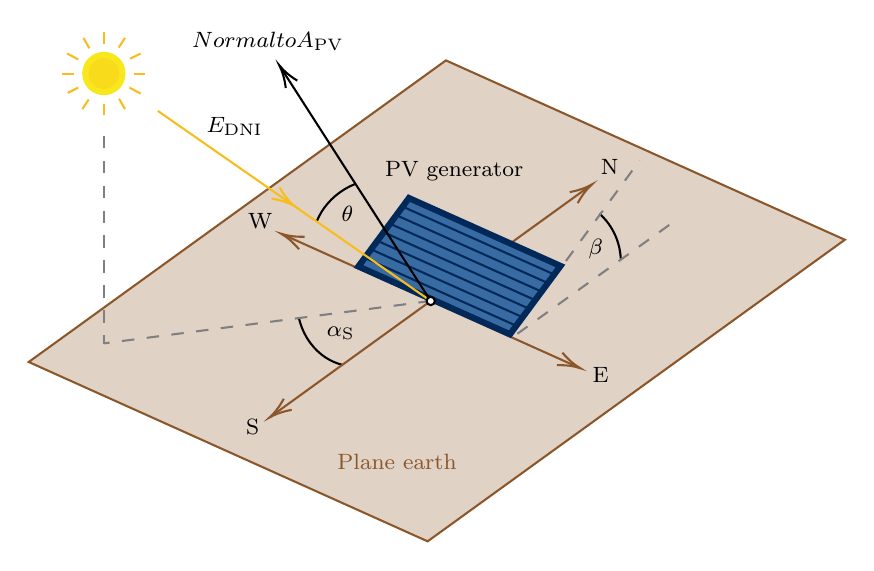
\begin{tikzpicture}[x=0.75pt,y=0.75pt,yscale=-1,xscale=1]
%uncomment if require: \path (0,455); %set diagram left start at 0, and has height of 455

%Shape: Rectangle [id:dp8474155302282593] 
\draw  [color={rgb, 255:red, 139; green, 87; blue, 42 }  ,draw opacity=1 ][fill={rgb, 255:red, 139; green, 87; blue, 42 }  ,fill opacity=0.27 ] (304.8,113.67) -- (496.99,200.08) -- (295.98,345.38) -- (103.79,258.97) -- cycle ;
%Straight Lines [id:da6680786992692076] 
\draw [color={rgb, 255:red, 139; green, 87; blue, 42 }  ,draw opacity=1 ]   (367.73,261.16) -- (227.22,197.98) ;
\draw [shift={(225.39,197.16)}, rotate = 384.21000000000004] [color={rgb, 255:red, 139; green, 87; blue, 42 }  ,draw opacity=1 ][line width=0.75]    (10.93,-3.29) .. controls (6.95,-1.4) and (3.31,-0.3) .. (0,0) .. controls (3.31,0.3) and (6.95,1.4) .. (10.93,3.29)   ;
\draw [shift={(369.56,261.98)}, rotate = 204.21] [color={rgb, 255:red, 139; green, 87; blue, 42 }  ,draw opacity=1 ][line width=0.75]    (10.93,-3.29) .. controls (6.95,-1.4) and (3.31,-0.3) .. (0,0) .. controls (3.31,0.3) and (6.95,1.4) .. (10.93,3.29)   ;
%Shape: Arc [id:dp4091032640411232] 
\draw  [draw opacity=0] (378.78,187.54) .. controls (381.04,189.51) and (383.04,191.89) .. (384.69,194.67) .. controls (387.37,199.17) and (388.78,204.17) .. (389.04,209.19) -- (360,211.71) -- cycle ; \draw   (378.78,187.54) .. controls (381.04,189.51) and (383.04,191.89) .. (384.69,194.67) .. controls (387.37,199.17) and (388.78,204.17) .. (389.04,209.19) ;
%Shape: Ellipse [id:dp7766653682919293] 
\draw  [color={rgb, 255:red, 248; green, 231; blue, 28 }  ,draw opacity=1 ][fill={rgb, 255:red, 248; green, 220; blue, 28 }  ,fill opacity=1 ][line width=2.25]  (131.06,120) .. controls (131.06,115.06) and (135.06,111.06) .. (140,111.06) .. controls (144.94,111.06) and (148.94,115.06) .. (148.94,120) .. controls (148.94,124.94) and (144.94,128.94) .. (140,128.94) .. controls (135.06,128.94) and (131.06,124.94) .. (131.06,120) -- cycle ;
%Straight Lines [id:da12322467795106329] 
\draw [color={rgb, 255:red, 248; green, 189; blue, 28 }  ,draw opacity=1 ]   (140,100) -- (140,105.56) ;
%Straight Lines [id:da4332784077616083] 
\draw [color={rgb, 255:red, 248; green, 189; blue, 28 }  ,draw opacity=1 ]   (160,120) -- (154.44,120) ;
%Straight Lines [id:da7027066659727501] 
\draw [color={rgb, 255:red, 248; green, 189; blue, 28 }  ,draw opacity=1 ]   (140,140) -- (140,134.44) ;
%Straight Lines [id:da11414191136971219] 
\draw [color={rgb, 255:red, 248; green, 189; blue, 28 }  ,draw opacity=1 ]   (125.56,120) -- (120,120) ;
%Straight Lines [id:da6688063172227983] 
\draw [color={rgb, 255:red, 248; green, 189; blue, 28 }  ,draw opacity=1 ]   (152.34,126.79) -- (157.7,129.65) ;
%Straight Lines [id:da20949775152165007] 
\draw [color={rgb, 255:red, 248; green, 189; blue, 28 }  ,draw opacity=1 ]   (122.3,110.35) -- (127.66,113.21) ;
%Straight Lines [id:da7656758253367213] 
\draw [color={rgb, 255:red, 248; green, 189; blue, 28 }  ,draw opacity=1 ]   (157.7,110.35) -- (152.65,112.85) ;
%Straight Lines [id:da9791803411373596] 
\draw [color={rgb, 255:red, 248; green, 189; blue, 28 }  ,draw opacity=1 ]   (127.66,126.79) -- (122.61,129.3) ;
%Straight Lines [id:da2234053647148624] 
\draw [color={rgb, 255:red, 248; green, 189; blue, 28 }  ,draw opacity=1 ]   (147.15,107.46) -- (150.19,102.84) ;
%Straight Lines [id:da6726326270351066] 
\draw [color={rgb, 255:red, 248; green, 189; blue, 28 }  ,draw opacity=1 ]   (129.63,137.14) -- (132.67,132.51) ;
%Straight Lines [id:da7766925486897012] 
\draw [color={rgb, 255:red, 248; green, 189; blue, 28 }  ,draw opacity=1 ]   (147.33,132.16) -- (150.19,137.16) ;
%Straight Lines [id:da3318298152117709] 
\draw [color={rgb, 255:red, 248; green, 189; blue, 28 }  ,draw opacity=1 ]   (130.17,102.84) -- (133.03,107.84) ;

%Straight Lines [id:da4654469204608218] 
\draw [color={rgb, 255:red, 128; green, 128; blue, 128 }  ,draw opacity=1 ] [dash pattern={on 4.5pt off 4.5pt}]  (140,150) -- (140,250.5) ;
%Shape: Arc [id:dp19974251160210033] 
\draw  [draw opacity=0] (255.22,260.43) .. controls (249.27,259.03) and (243.7,255.49) .. (239.53,249.88) .. controls (236.81,246.23) and (234.96,242.08) .. (233.96,237.75) -- (261.41,229.35) -- cycle ; \draw   (255.22,260.43) .. controls (249.27,259.03) and (243.7,255.49) .. (239.53,249.88) .. controls (236.81,246.23) and (234.96,242.08) .. (233.96,237.75) ;
%Straight Lines [id:da5130479264192895] 
\draw [color={rgb, 255:red, 139; green, 87; blue, 42 }  ,draw opacity=1 ]   (373.59,174.56) -- (221.36,284.59) ;
\draw [shift={(219.74,285.76)}, rotate = 324.14] [color={rgb, 255:red, 139; green, 87; blue, 42 }  ,draw opacity=1 ][line width=0.75]    (10.93,-3.29) .. controls (6.95,-1.4) and (3.31,-0.3) .. (0,0) .. controls (3.31,0.3) and (6.95,1.4) .. (10.93,3.29)   ;
\draw [shift={(375.21,173.38)}, rotate = 144.14] [color={rgb, 255:red, 139; green, 87; blue, 42 }  ,draw opacity=1 ][line width=0.75]    (10.93,-3.29) .. controls (6.95,-1.4) and (3.31,-0.3) .. (0,0) .. controls (3.31,0.3) and (6.95,1.4) .. (10.93,3.29)   ;
%Straight Lines [id:da7333561757823057] 
\draw [color={rgb, 255:red, 128; green, 128; blue, 128 }  ,draw opacity=1 ] [dash pattern={on 4.5pt off 4.5pt}]  (297.47,229.57) -- (140,250) ;
%Shape: Rectangle [id:dp9181904913709493] 
\draw  [color={rgb, 255:red, 0; green, 41; blue, 90 }  ,draw opacity=1 ][fill={rgb, 255:red, 57; green, 107; blue, 163 }  ,fill opacity=1 ][line width=2.25]  (286.99,180) -- (360,212.71) -- (335.66,245.63) -- (262.65,212.93) -- cycle ;
%Straight Lines [id:da13478383057933563] 
\draw [color={rgb, 255:red, 0; green, 41; blue, 90 }  ,draw opacity=1 ]   (283.95,184.12) -- (356.96,216.82) ;
%Straight Lines [id:da5884374823291068] 
\draw [color={rgb, 255:red, 0; green, 41; blue, 90 }  ,draw opacity=1 ]   (265.69,208.81) -- (338.7,241.52) ;
%Straight Lines [id:da02285619917411874] 
\draw [color={rgb, 255:red, 0; green, 41; blue, 90 }  ,draw opacity=1 ]   (268.74,204.7) -- (341.75,237.4) ;
%Straight Lines [id:da23820193833800274] 
\draw [color={rgb, 255:red, 0; green, 41; blue, 90 }  ,draw opacity=1 ]   (271.78,200.58) -- (344.79,233.28) ;
%Straight Lines [id:da14178706586084355] 
\draw [color={rgb, 255:red, 0; green, 41; blue, 90 }  ,draw opacity=1 ]   (280.9,188.23) -- (353.91,220.94) ;
%Straight Lines [id:da14421525428340431] 
\draw [color={rgb, 255:red, 0; green, 41; blue, 90 }  ,draw opacity=1 ]   (274.82,196.46) -- (347.83,229.17) ;
%Straight Lines [id:da3643942316695261] 
\draw [color={rgb, 255:red, 0; green, 41; blue, 90 }  ,draw opacity=1 ]   (277.86,192.35) -- (350.87,225.05) ;
%Shape: Arc [id:dp7190646059564607] 
\draw  [draw opacity=0] (242.59,191.14) .. controls (245.03,185.16) and (249.56,179.68) .. (255.82,175.84) .. controls (257.47,174.83) and (259.17,173.97) .. (260.9,173.27) -- (269.51,198.17) -- cycle ; \draw   (242.59,191.14) .. controls (245.03,185.16) and (249.56,179.68) .. (255.82,175.84) .. controls (257.47,174.83) and (259.17,173.97) .. (260.9,173.27) ;
%Straight Lines [id:da4133530859205612] 
\draw [color={rgb, 255:red, 248; green, 189; blue, 28 }  ,draw opacity=1 ][line width=0.75]    (166,138) -- (230.1,182.64) ;
\draw [shift={(231.74,183.79)}, rotate = 214.86] [color={rgb, 255:red, 248; green, 189; blue, 28 }  ,draw opacity=1 ][line width=0.75]    (10.93,-3.29) .. controls (6.95,-1.4) and (3.31,-0.3) .. (0,0) .. controls (3.31,0.3) and (6.95,1.4) .. (10.93,3.29)   ;
%Straight Lines [id:da8270043512595768] 
\draw [color={rgb, 255:red, 248; green, 189; blue, 28 }  ,draw opacity=1 ][line width=0.75]    (231.74,183.79) -- (297.47,229.57) ;
%Straight Lines [id:da7037472432355609] 
\draw [color={rgb, 255:red, 0; green, 0; blue, 0 }  ,draw opacity=1 ]   (297.47,229.57) -- (225.58,117.68) ;
\draw [shift={(224.5,116)}, rotate = 417.28] [color={rgb, 255:red, 0; green, 0; blue, 0 }  ,draw opacity=1 ][line width=0.75]    (10.93,-3.29) .. controls (6.95,-1.4) and (3.31,-0.3) .. (0,0) .. controls (3.31,0.3) and (6.95,1.4) .. (10.93,3.29)   ;
%Straight Lines [id:da7634900279620906] 
\draw [color={rgb, 255:red, 128; green, 128; blue, 128 }  ,draw opacity=1 ] [dash pattern={on 4.5pt off 4.5pt}]  (412.4,192.95) -- (334.66,248.63) ;
%Straight Lines [id:da3198763131888107] 
\draw [color={rgb, 255:red, 128; green, 128; blue, 128 }  ,draw opacity=1 ] [dash pattern={on 4.5pt off 4.5pt}]  (362.64,210.28) -- (398.15,161.88) ;
%Shape: Circle [id:dp009625788709507033] 
\draw  [fill={rgb, 255:red, 255; green, 255; blue, 255 }  ,fill opacity=1 ] (295.47,229.57) .. controls (295.47,228.47) and (296.37,227.57) .. (297.47,227.57) .. controls (298.58,227.57) and (299.47,228.47) .. (299.47,229.57) .. controls (299.47,230.68) and (298.58,231.57) .. (297.47,231.57) .. controls (296.37,231.57) and (295.47,230.68) .. (295.47,229.57) -- cycle ;

% Text Node
\draw (372,198.4) node [anchor=north west][inner sep=0.75pt]  [font=\footnotesize]  {$\beta $};
% Text Node
\draw (378,160) node [anchor=north west][inner sep=0.75pt]  [font=\footnotesize] [align=left] {N};
% Text Node
\draw (207,285) node [anchor=north west][inner sep=0.75pt]  [font=\footnotesize] [align=left] {S};
% Text Node
\draw (374,260) node [anchor=north west][inner sep=0.75pt]  [font=\footnotesize] [align=left] {E};
% Text Node
\draw (208,186) node [anchor=north west][inner sep=0.75pt]  [font=\footnotesize] [align=left] {W};
% Text Node
\draw (274,161) node [anchor=north west][inner sep=0.75pt]  [font=\footnotesize] [align=left] {PV generator};
% Text Node
\draw (246,240.4) node [anchor=north west][inner sep=0.75pt]  [font=\footnotesize]  {$\alpha _{\mathrm{S}}$};
% Text Node
\draw (253,182.4) node [anchor=north west][inner sep=0.75pt]  [font=\footnotesize]  {$\theta $};
% Text Node
\draw (251,302) node [anchor=north west][inner sep=0.75pt]  [font=\footnotesize,color={rgb, 255:red, 139; green, 87; blue, 42 }  ,opacity=1 ] [align=left] {Plane earth};
% Text Node
\draw (188,139.4) node [anchor=north west][inner sep=0.75pt]  [font=\footnotesize]  {$E_{\mathrm{DNI}}$};
% Text Node
\draw (181,98.4) node [anchor=north west][inner sep=0.75pt]  [font=\footnotesize]  {$\text{Normal to } A_{\mathrm{PV}}$};


\end{tikzpicture}

	\caption{Illustration of the incident angle $\theta$ of the solar rays. (Recreated from: \cite{Appelbaum:1993})}
	\label{fig:tikz_angle_theta}
\end{figure}
The angle on incident $\theta$, has the range $\left[0^\circ \text{, } 90^\circ\right]$. For completenes it must be mentioned, that equation \ref{eq:sin_gamma_s} can be derived from equation \ref{eq:cos_theta} with $\beta = 0^\circ$ and for $\gamma_{\mathrm{S}} + \beta = 90^\circ$ the Sun's rays are perpendicular to the PVG's surface area $A_{\mathrm{PVG}}$, which results in $E_{\mathrm{DGI}} = E_{\mathrm{DNI}}$ \cite{Appelbaum:1993, Mertens:2015, Wagner:2018}.

To determine the second component from eaquation \ref{eq:e_gen}, the sky is assumed to be isotropic. This means, that the DIFH is evenly distributed in the entire celestial hemisphere above the PVG. The more the PVG is inclined, the smaller the proportion of DIFG in equation \ref{eq:e_difg} becomes (compare to figure \ref{fig:tikz_three_component_model}) \cite{Appelbaum:1993, Mertens:2015}. 
\begin{center}
	\begin{equation} \label{eq:e_difg}
		E_{\mathrm{DIFG}} = E_{\mathrm{DIFH}} \, \frac{1 + \cos \beta }{2}
	\end{equation}
\end{center} 
In \cite{Mertens:2015} it is expressly pointed out that the isotropic approach used in equation \ref{eq:e_difg} is only a rough approximation. This is because the sky is brighter towards the Sun than towards the horizon.\footnote{More precise equations would be difficult to derive, which would go beyond the scope of this thesis.} 

When examining the last component from equtaion \ref{eq:e_gen}, it has to be taken into account, that different surfaces reflect solar radiation differently. In equation \ref{eq:e_rgi} this is accomplished with the factor $ALB$ -- also known as the albedo. Similar to equation \ref{eq:e_difg}, an isotropic approach is used \cite{Appelbaum:1993, Dobos:2003, Mertens:2015, Bralower:2018}. 
\begin{center}
	\begin{equation} \label{eq:e_rgi}
		E_{\mathrm{RGI}} = E_{\mathrm{GHI}} \, \frac{1 - \cos \beta }{2} \cdot ALB
	\end{equation}
\end{center}
Approximate albedo values for various surfaces are listed in table \ref{tab:table_albedo}. The larger the value, the more solar radiation is reflected. A blackbody for example, has an albedo value of 0 while an absolute white surface has an albedo value of 1. The Earth has an average albedo of 0,31 \cite{Dobos:2003, Bennett:2010, Bralower:2018}.

\begin{table}[h!]
	\centering
	\footnotesize
\begin{tabular}{|l|c|l|c|}
	\hline
	\textbf{Surface} & \textbf{Albedo} & \textbf{Surface} & \textbf{Albedo} \\
	\hline
	Forest & 0,05 -- 0,18 & Sand & 0,20 -- 0,40 \\
	Water & 0,06 -- 0,10 & Grass (July, August) & 0,25 \\
	Rain forest & 0,07 -- 0,15 & Dry sandy soil & 0,25 -- 0,45 \\
	Coniferous forest & 0,09 -- 0,15 & Uncultivated field & 0,26 \\
	Dark-colored soil surfaces & 0,10 -- 0,20 & New concrete & 0,30 \\
	Heathland & 0,10 -- 0,25 & Granite & 0,30 -- 0,35 \\
	Asphalt & 0,15 & Glacial ice & 0,30 -- 0,40 \\
	Deciduous forest & 0,15 -- 0,18 & Light-colored soil surfaces & 0,40 -- 0,50 \\
	Dry clay soil & 0,15 -- 0,35 & Old snow & 0,45 -- 0,70 \\
	Lawn & 0,18 -- 0,23 & Dry salt cover & 0,50 \\
	Weathered concrete & 0,20 & Fresh snow & 0,80 -- 0,90 \\
	\hline
\end{tabular}
	\caption{Albedo (refelctivity) values for different surfaces \cite{Dobos:2003, Bertol:2011, Mertens:2015, Bralower:2018}.}
	\label{tab:table_albedo}
\end{table}

If the three derived components $E_{\mathrm{DGI}}$, $E_{\mathrm{DIFG}}$ and $E_{\mathrm{RGI}}$ are now inserted into equation \ref{eq:e_gen} while considering equations \ref{eq:e_ghi} and \ref{eq:e_dni}, the total irradiance $E_{\mathrm{GEN}}$ received by an inclined PVG, depending on $E_{\mathrm{GHI}}$, $E_{\mathrm{DNI}}$, $\gamma_{\mathrm{S}}$ and its angle of inclination $\beta$, can be obtained \cite{Appelbaum:1992, Appelbaum:1993, Mertens:2015}:

\begin{center}
	\begin{equation} \label{eq:e_gen_ghi_dni}
		\begin{split}
		E_{\mathrm{GEN}} = E_{\mathrm{DNI}} \, \cos \theta + \left(E_{\mathrm{GHI}} - E_{\mathrm{DNI}} \, \sin \gamma_{\mathrm{S}}\right) \frac{1 + \cos \beta }{2} \\ 
		+ E_{\mathrm{GHI}} \, \frac{1 - \cos \beta }{2} \cdot ALB \text{.}
		\end{split}
	\end{equation}
\end{center}

Regarding this equation, it must be noted, that the angles $\gamma_{\mathrm{S}}$ and $\theta$ are time dependent and therefore the equation is time dependent. $E_{\mathrm{GHI}}$ and $E_{\mathrm{DNI}}$ on the other hand, are daily average values -- if taken from the solar resource maps shown previously -- and can therefore be treated as constants. And the angle of inclination $\beta$ as well as the albedo value $ALB$ are treated as constants as well. Because in theory, once the PVG of the self-sufficient BVCR is installed, its inclination angle $\beta$ will not change throughout the OeWF's mission. This has the consequence, that the PVG's inclined surface area $A_{\mathrm{PVG}}$ is only perpendicular for one pair of $\gamma_{\mathrm{S}}$ and $\alpha_{\mathrm{S}}$ at a given time of the day. 

And for completeness it should be mentioned, that even though $ALB$ is treated as a constant, there are situations, in which the albedo value of a surface can change drastically over the course of a few hours. For example if the PVG is installed on a freshly snowed uncultivated field and the snow melts away. In that case the $ALB$ would change from 0,80 down to 0,26. Such situations must be considered while simulating the PVG's daily energy yield, by for example simulating the worst case scenario.

As described by \cite{Mertens:2015, Wagner:2018}, the \emph{radiation flux} $\Phi_{\mathrm{GEN}}$ onto the PVG's surface area $A_{\mathrm{PVG}}$ -- to be more precise, the sum of the energy generating surface area of the PVG's solar cells -- can be calculated as follows:

\begin{center}
	\begin{equation} \label{eq:radiation_flux}
		\Phi_{\mathrm{GEN}} = A_{\mathrm{PVG}} \, E_{\mathrm{GEN}} \text{,}
	\end{equation}
\end{center}

How to determine the angle of inclination $\beta$ of the PVG, will be discussed in the next subsection.

%
%
%

%% Photovoltaic generator alignment %%

\subsection{Photovoltaic generator alignment} \label{sec:photovoltaic_generator_alignment}
The Sun's direct irradiance for clear skies reaches its greates daily value at solar noon for $t_{\mathrm{S}} = 12\mathrm{h}$. This is the point in time, in which $\gamma_{\mathrm{S}}$ reaches its greates daily value as well, and thus the Sun's rays have the shortest path through the Earth's atmosphere to the surface. It is longer, the smaller $\gamma_{\mathrm{S}}$ becomes -- regardless of whether it is before or after solar noon.\footnote{Regarding the optimal angles of a PVG for clear skies, the authors of \cite{Appelbaum:1993} write: \begin{displayquote}\textit{"For clear days, the solar irradiance is symmetrical around noon and is maximum at true solar noon, $\omega = 0$."}\end{displayquote} With $\omega$ being the solar hour angle $h_{\mathrm{S}}$.} The factor responsible for this is the air mass (AM) value $x$ \cite{Appelbaum:1993, Bertol:2011, Mertens:2015, Wagner:2018}:

\begin{center}
	\begin{equation} \label{eq:air_mass}
		x = \frac{1}{\sin \gamma_{\mathrm{S}}} \text{.}
	\end{equation}
\end{center}

For example, for $\gamma_{\mathrm{S}} = 90^\circ$ the Sun is at its zenith and therefore its rays have the shortest possible path through the Earth's atmosphere to the surface. And since the spectrum of the Sun on Earth's surface changes, depending on the length of the path of the Sun's rays, this spectrum is called AM1 spectrum. The AM0 specturm would be outside the Earth's atmosphere which corresponds to the previously mentioned solar constant $E_{\mathrm{S}}$ \cite{Mertens:2015, Wagner:2018}. 

Besides this, the self-sufficent BVCR and therefore the PVG will be in use for the entire duration of the OeWF's missions -- in other words, it is constantly active and therefore needs energy throughout the day.

Based on these findings it can be said, that a stationary PVG must be aligned in a way, that its suface area $A_{\mathrm{PVG}}$ is perpendicular to the Sun's rays when it reaches its greates daily irradiance value -- so the normal to $A_{\mathrm{PVG}}$ aligns with the incoming rays. In this way it can achieve maximum daily energy yield. With stationary it is meant, that the PVG does not actively track the Sun throughout the day, but is installed with a fixed orientation of the normal to $A_{\mathrm{PVG}}$ and a constant inclination angle $\beta$ \cite{Appelbaum:1993, Mertens:2015, Wagner:2018}.

As mentioned in subsection \ref{sec:energy_yield}, the Sun's rays are perpendicular to the surface area $A_{\mathrm{PVG}}$ for $\beta = 90^\circ - \gamma_{\mathrm{S}}$. After applying this to equation \ref{eq:sin_gamma_s} and simplifying it with trigonometric functions (see appendix \ref{sec:trigonometry}), the PVG's angle of inclinations $\beta$ at a latitude $\varphi$, with Earth's axis of rotation inclined towards the Sun with the angle $\delta$, can be derived as shown in equation \ref{eq:beta_with_delta_and_phi} \cite{Appelbaum:1993, Mertens:2015, Wagner:2018}.

\begin{center}
	\begin{equation} \label{eq:beta_with_delta_and_phi}
		\beta = \varphi - \delta
	\end{equation}
\end{center}

Determining how the normal to $A_{\mathrm{PVG}}$ must be oriented, is accomplished by using the equations \ref{eq:sin_gamma_s} and \ref{eq:cos_alpha_s}, and solving them for $t_{\mathrm{S}} = 12\mathrm{h}$. With the help of trigonometric functions (see appendix \ref{sec:trigonometry}), this results in:

\begin{center}
	\begin{equation} \label{eq:gamma_s_align}
		\gamma_{\mathrm{S}} = 90^\circ - \varphi + \delta \text{,} \quad \text{for } t_{\mathrm{S}} = 12\mathrm{h}
	\end{equation}
\end{center}

\begin{center}
	\begin{equation} \label{eq:alpha_s_align}
		\alpha_{\mathrm{S}} = \arcsin \left(\frac{\sin \left(\varphi - \delta\right)}{\cos \gamma_{\mathrm{S}}}\right) \text{,} \quad \text{for } t_{\mathrm{S}} = 12\mathrm{h} \text{.}
	\end{equation}
\end{center}

For $\alpha_{\mathrm{S}} = 0^\circ$ the Sun is visible in the south and therefore the PVG must be oriented in a way, so that the normal to $A_{\mathrm{PVG}}$ points towards the south. And for $\alpha_{\mathrm{S}} = 180^\circ$ the Sun is visible in the north and therefore the normal to $A_{\mathrm{PVG}}$ must point towards the north. For the last possible case, when the Sun is at its zenith, $\alpha_{\mathrm{S}}$ cannot be solved, because $\gamma_{\mathrm{S}} = 90^\circ$.

A more practical approach to this can be achieved by comparing the latitude of the PVG's installation site, to the latitude $\varphi_{\mathrm{Z}}$ where the Sun is at its zenith for $t_{\mathrm{S}} = 12\mathrm{h}$, using a GPS device. Figure \ref{fig:crucial_latitudes} compares the three different cases of the Sun's location in the sky, depending on the installation site of the PVG, in which $\varphi_{\mathrm{S}}$ is an installation site to the south and $\varphi_{\mathrm{N}}$ to the north of $\varphi_{\mathrm{Z}}$.

\begin{figure}[h!]
	\centering
		\begin{subfigure}[b]{0.3\linewidth}
			

\tikzset{every picture/.style={line width=0.75pt}} %set default line width to 0.75pt        

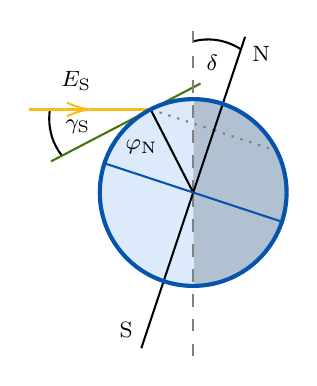
\begin{tikzpicture}[x=0.75pt,y=0.75pt,yscale=-1,xscale=1]
%uncomment if require: \path (0,201); %set diagram left start at 0, and has height of 201

%Shape: Pie [id:dp4750642586964353] 
\draw  [color={rgb, 255:red, 0; green, 0; blue, 0 }  ,draw opacity=0 ][fill={rgb, 255:red, 0; green, 0; blue, 0 }  ,fill opacity=0.45 ] (93.03,60.03) .. controls (117.81,60.3) and (137.85,80.25) .. (137.93,104.89) .. controls (138.02,129.63) and (117.94,149.78) .. (93.03,150.05) -- (92.52,105.04) -- cycle ;
%Shape: Circle [id:dp9006978183202985] 
\draw  [color={rgb, 255:red, 7; green, 84; blue, 173 }  ,draw opacity=1 ][fill={rgb, 255:red, 200; green, 222; blue, 248 }  ,fill opacity=0.64 ][line width=0.75]  (47.52,105.04) .. controls (47.52,80.19) and (67.67,60.04) .. (92.52,60.04) .. controls (117.38,60.04) and (137.52,80.19) .. (137.52,105.04) .. controls (137.52,129.89) and (117.38,150.04) .. (92.52,150.04) .. controls (67.67,150.04) and (47.52,129.89) .. (47.52,105.04) -- cycle ;
%Straight Lines [id:da06282467353758259] 
\draw [color={rgb, 255:red, 65; green, 117; blue, 5 }  ,draw opacity=1 ]   (96.02,52.54) -- (72.02,65.04) ;
%Shape: Arc [id:dp49173933797962777] 
\draw  [draw opacity=0] (29.42,87.46) .. controls (28.29,86.06) and (27.29,84.54) .. (26.43,82.91) .. controls (23.51,77.38) and (22.61,71.21) .. (23.45,65.01) -- (66.02,62.04) -- cycle ; \draw   (29.42,87.46) .. controls (28.29,86.06) and (27.29,84.54) .. (26.43,82.91) .. controls (23.51,77.38) and (22.61,71.21) .. (23.45,65.01) ;
%Straight Lines [id:da6550544250175496] 
\draw [color={rgb, 255:red, 65; green, 117; blue, 5 }  ,draw opacity=1 ]   (24.02,90.04) -- (72.02,65.04) ;
%Shape: Arc [id:dp963370582460114] 
\draw  [draw opacity=0] (92.23,32.3) .. controls (94.76,31.6) and (97.38,31.25) .. (100.07,31.29) .. controls (105.67,31.35) and (110.94,33.08) .. (115.6,36.08) -- (99.52,76.04) -- cycle ; \draw   (92.23,32.3) .. controls (94.76,31.6) and (97.38,31.25) .. (100.07,31.29) .. controls (105.67,31.35) and (110.94,33.08) .. (115.6,36.08) ;
%Straight Lines [id:da058893605247020586] 
\draw [color={rgb, 255:red, 128; green, 128; blue, 128 }  ,draw opacity=1 ] [dash pattern={on 4.5pt off 4.5pt}]  (92.52,183.96) -- (92.52,105.04) ;
%Straight Lines [id:da5478983474017609] 
\draw [color={rgb, 255:red, 128; green, 128; blue, 128 }  ,draw opacity=1 ] [dash pattern={on 4.5pt off 4.5pt}]  (92.52,105.04) -- (92.52,26.12) ;
%Straight Lines [id:da4780085054484584] 
\draw [line width=0.75]    (72.02,65.04) -- (92.52,105.04) ;
%Straight Lines [id:da5291514924825897] 
\draw [color={rgb, 255:red, 128; green, 128; blue, 128 }  ,draw opacity=1 ] [dash pattern={on 0.84pt off 2.51pt}]  (102.52,75.04) -- (133.02,85.04) ;
%Straight Lines [id:da4294056374442512] 
\draw [color={rgb, 255:red, 128; green, 128; blue, 128 }  ,draw opacity=1 ] [dash pattern={on 0.84pt off 2.51pt}]  (72.02,65.04) -- (102.52,75.04) ;
%Straight Lines [id:da35119327320040794] 
\draw    (92.52,105.04) -- (67.52,180.04) ;
%Straight Lines [id:da9687000233514724] 
\draw    (117.52,30.04) -- (92.52,105.04) ;
%Straight Lines [id:da8818616046820387] 
\draw [color={rgb, 255:red, 7; green, 84; blue, 173 }  ,draw opacity=1 ]   (50.02,91.04) -- (92.52,105.04) ;
%Straight Lines [id:da4795343191360564] 
\draw [color={rgb, 255:red, 7; green, 84; blue, 173 }  ,draw opacity=1 ]   (92.52,105.04) -- (135.02,119.04) ;
%Straight Lines [id:da6396043564859444] 
\draw [color={rgb, 255:red, 248; green, 189; blue, 28 }  ,draw opacity=1 ]   (42.65,65.04) -- (72.02,65.04) ;
%Straight Lines [id:da3150442288480175] 
\draw [color={rgb, 255:red, 248; green, 189; blue, 28 }  ,draw opacity=1 ]   (13.27,65.04) -- (40.65,65.04) ;
\draw [shift={(42.65,65.04)}, rotate = 180] [color={rgb, 255:red, 248; green, 189; blue, 28 }  ,draw opacity=1 ][line width=0.75]    (10.93,-3.29) .. controls (6.95,-1.4) and (3.31,-0.3) .. (0,0) .. controls (3.31,0.3) and (6.95,1.4) .. (10.93,3.29)   ;
%Shape: Circle [id:dp4877206756511603] 
\draw  [color={rgb, 255:red, 7; green, 84; blue, 173 }  ,draw opacity=1 ][fill={rgb, 255:red, 200; green, 222; blue, 248 }  ,fill opacity=0 ][line width=1.5]  (47.52,105.04) .. controls (47.52,80.19) and (67.67,60.04) .. (92.52,60.04) .. controls (117.38,60.04) and (137.52,80.19) .. (137.52,105.04) .. controls (137.52,129.89) and (117.38,150.04) .. (92.52,150.04) .. controls (67.67,150.04) and (47.52,129.89) .. (47.52,105.04) -- cycle ;

% Text Node
\draw (58.52,78.4) node [anchor=north west][inner sep=0.75pt]  [font=\footnotesize]  {$\varphi _{\mathrm{N}}$};
% Text Node
\draw (97.52,37.44) node [anchor=north west][inner sep=0.75pt]  [font=\footnotesize]  {$\delta $};
% Text Node
\draw (29.52,68.44) node [anchor=north west][inner sep=0.75pt]  [font=\footnotesize]  {$\gamma _{\mathrm{S}}$};
% Text Node
\draw (27.52,45.4) node [anchor=north west][inner sep=0.75pt]  [font=\footnotesize]  {$E_{\mathrm{S}}$};
% Text Node
\draw (119.52,33.04) node [anchor=north west][inner sep=0.75pt]  [font=\footnotesize] [align=left] {N};
% Text Node
\draw (55.52,166.04) node [anchor=north west][inner sep=0.75pt]  [font=\footnotesize] [align=left] {S};


\end{tikzpicture}

			\caption{Northern latitude.}
		\end{subfigure}
		\begin{subfigure}[b]{0.3\linewidth}
			

\tikzset{every picture/.style={line width=0.75pt}} %set default line width to 0.75pt        

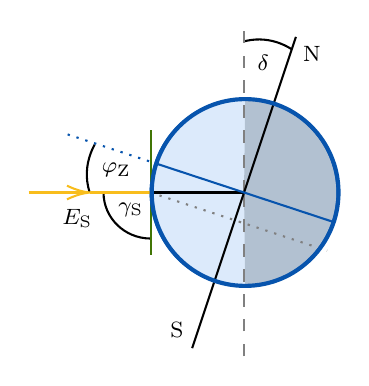
\begin{tikzpicture}[x=0.75pt,y=0.75pt,yscale=-1,xscale=1]
%uncomment if require: \path (0,181); %set diagram left start at 0, and has height of 181

%Shape: Arc [id:dp20953347708018688] 
\draw  [draw opacity=0] (69.43,111.09) .. controls (69.33,111.09) and (69.24,111.09) .. (69.15,111.09) .. controls (56.73,110.92) and (46.77,101.07) .. (46.73,89) -- (69.44,88.92) -- cycle ; \draw   (69.43,111.09) .. controls (69.33,111.09) and (69.24,111.09) .. (69.15,111.09) .. controls (56.73,110.92) and (46.77,101.07) .. (46.73,89) ;
%Shape: Arc [id:dp16591242877449974] 
\draw  [draw opacity=0] (40.06,88.92) .. controls (39.51,87.21) and (39.11,85.44) .. (38.89,83.61) .. controls (38.13,77.4) and (39.47,71.31) .. (42.46,65.81) -- (83.31,78.18) -- cycle ; \draw   (40.06,88.92) .. controls (39.51,87.21) and (39.11,85.44) .. (38.89,83.61) .. controls (38.13,77.4) and (39.47,71.31) .. (42.46,65.81) ;
%Straight Lines [id:da6013522376382066] 
\draw [color={rgb, 255:red, 65; green, 117; blue, 5 }  ,draw opacity=1 ]   (69.44,118.92) -- (69.44,88.92) ;
%Shape: Pie [id:dp028486029029515914] 
\draw  [color={rgb, 255:red, 0; green, 0; blue, 0 }  ,draw opacity=0 ][fill={rgb, 255:red, 0; green, 0; blue, 0 }  ,fill opacity=0.45 ] (114.95,43.91) .. controls (139.73,44.18) and (159.77,64.13) .. (159.85,88.77) .. controls (159.93,113.51) and (139.86,133.66) .. (114.94,133.93) -- (114.44,88.92) -- cycle ;
%Shape: Circle [id:dp7286185522053927] 
\draw  [color={rgb, 255:red, 7; green, 84; blue, 173 }  ,draw opacity=1 ][fill={rgb, 255:red, 200; green, 222; blue, 248 }  ,fill opacity=0.64 ][line width=0.75]  (69.44,88.92) .. controls (69.44,64.07) and (89.59,43.92) .. (114.44,43.92) .. controls (139.29,43.92) and (159.44,64.07) .. (159.44,88.92) .. controls (159.44,113.77) and (139.29,133.92) .. (114.44,133.92) .. controls (89.59,133.92) and (69.44,113.77) .. (69.44,88.92) -- cycle ;
%Shape: Arc [id:dp17913789171454497] 
\draw  [draw opacity=0] (114.15,16.18) .. controls (116.67,15.49) and (119.3,15.14) .. (121.99,15.17) .. controls (127.58,15.24) and (132.85,16.96) .. (137.52,19.97) -- (121.44,59.92) -- cycle ; \draw   (114.15,16.18) .. controls (116.67,15.49) and (119.3,15.14) .. (121.99,15.17) .. controls (127.58,15.24) and (132.85,16.96) .. (137.52,19.97) ;
%Straight Lines [id:da9967059081670446] 
\draw [color={rgb, 255:red, 128; green, 128; blue, 128 }  ,draw opacity=1 ] [dash pattern={on 4.5pt off 4.5pt}]  (114.44,167.84) -- (114.44,88.92) ;
%Straight Lines [id:da71597890822506] 
\draw [color={rgb, 255:red, 128; green, 128; blue, 128 }  ,draw opacity=1 ] [dash pattern={on 4.5pt off 4.5pt}]  (114.44,88.92) -- (114.44,10) ;
%Straight Lines [id:da4137878061890663] 
\draw [color={rgb, 255:red, 128; green, 128; blue, 128 }  ,draw opacity=1 ] [dash pattern={on 0.84pt off 2.51pt}]  (69.44,88.92) -- (111.94,102.92) ;
%Straight Lines [id:da3390187694217488] 
\draw [color={rgb, 255:red, 128; green, 128; blue, 128 }  ,draw opacity=1 ] [dash pattern={on 0.84pt off 2.51pt}]  (111.94,102.92) -- (154.44,116.92) ;
%Straight Lines [id:da5052190602488993] 
\draw    (114.44,88.92) -- (89.44,163.92) ;
%Straight Lines [id:da6983846735857875] 
\draw    (139.44,13.92) -- (114.44,88.92) ;
%Straight Lines [id:da5175201690882127] 
\draw    (69.44,88.92) -- (114.44,88.92) ;
%Straight Lines [id:da23163800871480023] 
\draw [color={rgb, 255:red, 65; green, 117; blue, 5 }  ,draw opacity=1 ]   (69.44,88.92) -- (69.44,58.92) ;
%Straight Lines [id:da47404926603772557] 
\draw [color={rgb, 255:red, 7; green, 84; blue, 173 }  ,draw opacity=1 ] [dash pattern={on 0.84pt off 2.51pt}]  (29.44,60.92) -- (71.94,74.92) ;
%Straight Lines [id:da6548182479176137] 
\draw [color={rgb, 255:red, 248; green, 189; blue, 28 }  ,draw opacity=1 ]   (10.69,88.92) -- (38.06,88.92) ;
\draw [shift={(40.06,88.92)}, rotate = 180] [color={rgb, 255:red, 248; green, 189; blue, 28 }  ,draw opacity=1 ][line width=0.75]    (10.93,-3.29) .. controls (6.95,-1.4) and (3.31,-0.3) .. (0,0) .. controls (3.31,0.3) and (6.95,1.4) .. (10.93,3.29)   ;
%Straight Lines [id:da7518207882403078] 
\draw [color={rgb, 255:red, 248; green, 189; blue, 28 }  ,draw opacity=1 ]   (40.06,88.92) -- (69.44,88.92) ;
%Shape: Circle [id:dp4417291051670942] 
\draw  [color={rgb, 255:red, 7; green, 84; blue, 173 }  ,draw opacity=1 ][fill={rgb, 255:red, 200; green, 222; blue, 248 }  ,fill opacity=0 ][line width=1.5]  (69.95,88.91) .. controls (69.95,64.06) and (90.1,43.91) .. (114.95,43.91) .. controls (139.8,43.91) and (159.95,64.06) .. (159.95,88.91) .. controls (159.95,113.77) and (139.8,133.91) .. (114.95,133.91) .. controls (90.1,133.91) and (69.95,113.77) .. (69.95,88.91) -- cycle ;
%Straight Lines [id:da09584357360735729] 
\draw [color={rgb, 255:red, 7; green, 84; blue, 173 }  ,draw opacity=1 ]   (71.94,74.92) -- (114.44,88.92) ;
%Straight Lines [id:da1322107965109387] 
\draw [color={rgb, 255:red, 7; green, 84; blue, 173 }  ,draw opacity=1 ]   (114.44,88.92) -- (156.94,102.92) ;

% Text Node
\draw (44.44,73.32) node [anchor=north west][inner sep=0.75pt]  [font=\footnotesize]  {$\varphi _{\mathrm{Z}}$};
% Text Node
\draw (119.44,21.32) node [anchor=north west][inner sep=0.75pt]  [font=\footnotesize]  {$\delta $};
% Text Node
\draw (25.44,95.4) node [anchor=north west][inner sep=0.75pt]  [font=\footnotesize]  {$E_{\mathrm{S}}$};
% Text Node
\draw (141.44,16.92) node [anchor=north west][inner sep=0.75pt]  [font=\footnotesize] [align=left] {N};
% Text Node
\draw (77.44,149.92) node [anchor=north west][inner sep=0.75pt]  [font=\footnotesize] [align=left] {S};
% Text Node
\draw (52.44,92.32) node [anchor=north west][inner sep=0.75pt]  [font=\footnotesize]  {$\gamma _{\mathrm{S}}$};


\end{tikzpicture}

			\caption{Sun is at its zenith.}
		\end{subfigure}
		\begin{subfigure}[b]{0.3\linewidth}
			

\tikzset{every picture/.style={line width=0.75pt}} %set default line width to 0.75pt        

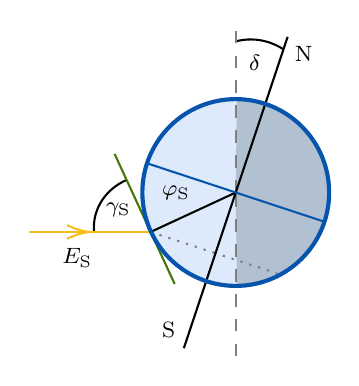
\begin{tikzpicture}[x=0.75pt,y=0.75pt,yscale=-1,xscale=1]
%uncomment if require: \path (0,181); %set diagram left start at 0, and has height of 181

%Shape: Arc [id:dp1509931683753729] 
\draw  [draw opacity=0] (41.51,107.98) .. controls (41.44,107.22) and (41.4,106.45) .. (41.4,105.68) .. controls (41.4,95.62) and (47.84,86.94) .. (57.17,82.86) -- (69.17,105.68) -- cycle ; \draw   (41.51,107.98) .. controls (41.44,107.22) and (41.4,106.45) .. (41.4,105.68) .. controls (41.4,95.62) and (47.84,86.94) .. (57.17,82.86) ;
%Shape: Pie [id:dp008234319355738817] 
\draw  [color={rgb, 255:red, 0; green, 0; blue, 0 }  ,draw opacity=0 ][fill={rgb, 255:red, 0; green, 0; blue, 0 }  ,fill opacity=0.45 ] (110.26,43.91) .. controls (135.04,44.18) and (155.08,64.13) .. (155.16,88.77) .. controls (155.24,113.51) and (135.17,133.66) .. (110.25,133.93) -- (109.75,88.92) -- cycle ;
%Shape: Circle [id:dp3321431212746069] 
\draw  [color={rgb, 255:red, 7; green, 84; blue, 173 }  ,draw opacity=1 ][fill={rgb, 255:red, 200; green, 222; blue, 248 }  ,fill opacity=0.64 ][line width=0.75]  (64.75,88.92) .. controls (64.75,64.07) and (84.9,43.92) .. (109.75,43.92) .. controls (134.6,43.92) and (154.75,64.07) .. (154.75,88.92) .. controls (154.75,113.77) and (134.6,133.92) .. (109.75,133.92) .. controls (84.9,133.92) and (64.75,113.77) .. (64.75,88.92) -- cycle ;
%Straight Lines [id:da8319048303736489] 
\draw [color={rgb, 255:red, 65; green, 117; blue, 5 }  ,draw opacity=1 ]   (57.17,82.86) -- (68.75,107.92) ;
%Shape: Arc [id:dp7416942399851174] 
\draw  [draw opacity=0] (109.46,16.18) .. controls (111.99,15.49) and (114.61,15.14) .. (117.3,15.17) .. controls (122.89,15.24) and (128.16,16.96) .. (132.83,19.97) -- (116.75,59.92) -- cycle ; \draw   (109.46,16.18) .. controls (111.99,15.49) and (114.61,15.14) .. (117.3,15.17) .. controls (122.89,15.24) and (128.16,16.96) .. (132.83,19.97) ;
%Straight Lines [id:da23785833539369183] 
\draw [color={rgb, 255:red, 128; green, 128; blue, 128 }  ,draw opacity=1 ] [dash pattern={on 4.5pt off 4.5pt}]  (109.75,167.84) -- (109.75,88.92) ;
%Straight Lines [id:da06972248148475568] 
\draw [color={rgb, 255:red, 128; green, 128; blue, 128 }  ,draw opacity=1 ] [dash pattern={on 4.5pt off 4.5pt}]  (109.75,88.92) -- (109.75,10) ;
%Straight Lines [id:da8960602024330377] 
\draw [line width=0.75]    (68.75,107.92) -- (109.75,88.92) ;
%Straight Lines [id:da5098060920131091] 
\draw [color={rgb, 255:red, 128; green, 128; blue, 128 }  ,draw opacity=1 ] [dash pattern={on 0.84pt off 2.51pt}]  (99.25,117.92) -- (129.75,127.92) ;
%Straight Lines [id:da8906380552334501] 
\draw [color={rgb, 255:red, 128; green, 128; blue, 128 }  ,draw opacity=1 ] [dash pattern={on 0.84pt off 2.51pt}]  (68.75,107.92) -- (99.25,117.92) ;
%Straight Lines [id:da14349690184184327] 
\draw    (109.75,88.92) -- (84.75,163.92) ;
%Straight Lines [id:da024036142327008347] 
\draw    (134.75,13.92) -- (109.75,88.92) ;
%Straight Lines [id:da21245027564913532] 
\draw [color={rgb, 255:red, 7; green, 84; blue, 173 }  ,draw opacity=1 ]   (67.25,74.92) -- (109.75,88.92) ;
%Straight Lines [id:da7748765899346521] 
\draw [color={rgb, 255:red, 7; green, 84; blue, 173 }  ,draw opacity=1 ]   (109.75,88.92) -- (152.25,102.92) ;
%Straight Lines [id:da645165483038932] 
\draw [color={rgb, 255:red, 65; green, 117; blue, 5 }  ,draw opacity=1 ]   (68.75,107.92) -- (80.33,132.98) ;
%Straight Lines [id:da01702325380082992] 
\draw [color={rgb, 255:red, 65; green, 117; blue, 5 }  ,draw opacity=1 ]   (57.17,82.86) -- (51.38,70.33) ;
%Straight Lines [id:da7674893611261671] 
\draw [color={rgb, 255:red, 248; green, 189; blue, 28 }  ,draw opacity=1 ]   (39.38,107.92) -- (68.75,107.92) ;
%Straight Lines [id:da5473156330354862] 
\draw [color={rgb, 255:red, 248; green, 189; blue, 28 }  ,draw opacity=1 ]   (10,107.92) -- (37.38,107.92) ;
\draw [shift={(39.38,107.92)}, rotate = 180] [color={rgb, 255:red, 248; green, 189; blue, 28 }  ,draw opacity=1 ][line width=0.75]    (10.93,-3.29) .. controls (6.95,-1.4) and (3.31,-0.3) .. (0,0) .. controls (3.31,0.3) and (6.95,1.4) .. (10.93,3.29)   ;
%Shape: Circle [id:dp46167221588038543] 
\draw  [color={rgb, 255:red, 7; green, 84; blue, 173 }  ,draw opacity=1 ][fill={rgb, 255:red, 200; green, 222; blue, 248 }  ,fill opacity=0 ][line width=1.5]  (64.75,88.92) .. controls (64.75,64.07) and (84.9,43.92) .. (109.75,43.92) .. controls (134.6,43.92) and (154.75,64.07) .. (154.75,88.92) .. controls (154.75,113.77) and (134.6,133.92) .. (109.75,133.92) .. controls (84.9,133.92) and (64.75,113.77) .. (64.75,88.92) -- cycle ;

% Text Node
\draw (72.75,84.32) node [anchor=north west][inner sep=0.75pt]  [font=\footnotesize]  {$\varphi _{\mathrm{S}}$};
% Text Node
\draw (114.75,21.32) node [anchor=north west][inner sep=0.75pt]  [font=\footnotesize]  {$\delta $};
% Text Node
\draw (45.75,92.32) node [anchor=north west][inner sep=0.75pt]  [font=\footnotesize]  {$\gamma _{\mathrm{S}}$};
% Text Node
\draw (24.75,114.32) node [anchor=north west][inner sep=0.75pt]  [font=\footnotesize]  {$E_{\mathrm{S}}$};
% Text Node
\draw (136.75,16.92) node [anchor=north west][inner sep=0.75pt]  [font=\footnotesize] [align=left] {N};
% Text Node
\draw (72.75,149.92) node [anchor=north west][inner sep=0.75pt]  [font=\footnotesize] [align=left] {S};


\end{tikzpicture}

			\caption{Southern latitude.}
		\end{subfigure}
	\caption{Illustration of the latitude $\varphi_{\mathrm{Z}}$ on Earth, which determines if a photovoltaic generator should be aligned to the north or to the south.}
	\label{fig:crucial_latitudes}
\end{figure}

Using equation \ref{eq:sin_gamma_s} for $\gamma_{\mathrm{S}} = 90^\circ$ and $t_{\mathrm{S}} = 12\mathrm{h}$ -- after applying trigonometric functions from appendix \ref{sec:trigonometry} -- the latitude $\varphi_{\mathrm{Z}}$ can be determined to:
\begin{center}
	\begin{equation} \label{eq:phi_z}
		\varphi_{\mathrm{Z}} = \delta \text{.}
	\end{equation}
\end{center}
If a PVG is installed at a latitude south of $\varphi_{\mathrm{Z}}$, the normal to $A_{\mathrm{PVG}}$ must point towards the north and if it is installed north of $\varphi_{\mathrm{Z}}$ the normal to $A_{\mathrm{PVG}}$ must point towards the south. In case the PVG is set up at the latitude $\varphi_{\mathrm{Z}}$ it does not matter how it is aligned because $\beta = \varphi_{\mathrm{Z}} - \delta = 0^\circ$, which means, that the PVG lays flat on plane earth. For completeness it shall be mentioned, that the normal to $A_{\mathrm{PVG}}$ can be aligned using a simple compass.

%
%
%

%% Modeling the solar radiation curve %%

\subsection{Modeling the solar energy curve} \label{sec:solar_energy_curve}
To estimte the behavior of a PVG, inclined with the angle $\beta$, the Sun's radiation flux $\Phi_{\mathrm{GEN}}$ onto its surface area $A_{\mathrm{PVG}}$ over the course of one day, must be simulated. Since the Sun's irradiance is symmetrical for $t_0 = 12\mathrm{h}$, and the PVG is assumed to be aligned, so that $A_{\mathrm{PVG}}$ is perpendicular to the Sun's rays for $t_0 = 12\mathrm{h}$, the Sun's radiation flux $\Phi_{\mathrm{GEN}}$, as a Gaussian function of the solar time $t_{\mathrm{S}}$, can be approximated as shown in figure \ref{fig:tikz_energy_gauss} \cite{Appelbaum:1993}.

\begin{figure}[h!]
	\centering
	

\tikzset{every picture/.style={line width=0.75pt}} %set default line width to 0.75pt        

\begin{tikzpicture}[x=0.75pt,y=0.75pt,yscale=-1,xscale=1]
%uncomment if require: \path (0,300); %set diagram left start at 0, and has height of 300

%Image [id:dp32150908690987645] 
\draw (327,150) node  {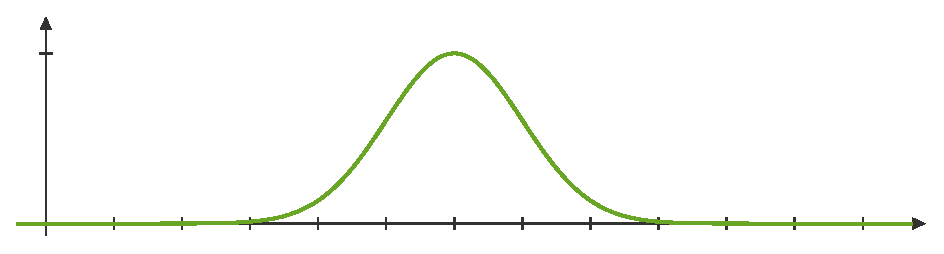
\includegraphics[width=439.5pt,height=105pt]{images/image_energy_gauss}};
%Straight Lines [id:da07666169968429992] 
\draw [color={rgb, 255:red, 155; green, 155; blue, 155 }  ,draw opacity=1 ] [dash pattern={on 4.5pt off 4.5pt}]  (63,103.4) -- (306,103.4) ;
%Straight Lines [id:da12384412498194441] 
\draw [color={rgb, 255:red, 155; green, 155; blue, 155 }  ,draw opacity=1 ] [dash pattern={on 4.5pt off 4.5pt}]  (315.6,201) -- (315.6,103) ;
%Shape: Circle [id:dp581375357919033] 
\draw  [fill={rgb, 255:red, 255; green, 255; blue, 255 }  ,fill opacity=1 ] (313.6,103.5) .. controls (313.6,102.4) and (314.5,101.5) .. (315.6,101.5) .. controls (316.7,101.5) and (317.6,102.4) .. (317.6,103.5) .. controls (317.6,104.6) and (316.7,105.5) .. (315.6,105.5) .. controls (314.5,105.5) and (313.6,104.6) .. (313.6,103.5) -- cycle ;

% Text Node
\draw (626,205.4) node [anchor=north west][inner sep=0.75pt]  [font=\footnotesize]  {$t_{\mathrm{S}}$};
% Text Node
\draw (34,59.4) node [anchor=north west][inner sep=0.75pt]  [font=\footnotesize]  {$\Phi _{\mathrm{G}}( t_{\mathrm{S}})$};
% Text Node
\draw (15,97.4) node [anchor=north west][inner sep=0.75pt]  [font=\footnotesize]  {$\Phi _{\mathrm{max}}$};
% Text Node
\draw (143,220.4) node [anchor=north west][inner sep=0.75pt]  [font=\footnotesize]  {$t_{\mathrm{S,r}} =t_{0} -3\tau _{\mathrm{S}}$};
% Text Node
\draw (162,240) node [anchor=north west][inner sep=0.75pt]  [font=\footnotesize] [align=left] {Sunrise};
% Text Node
\draw (298,240) node [anchor=north west][inner sep=0.75pt]  [font=\footnotesize] [align=left] {Noon};
% Text Node
\draw (287.5,220.4) node [anchor=north west][inner sep=0.75pt]  [font=\footnotesize]  {$t_{0} =12\mathrm{h}$};
% Text Node
\draw (403.1,220.4) node [anchor=north west][inner sep=0.75pt]  [font=\footnotesize]  {$t_{\mathrm{S,s}} =t_{0} +3\tau _{\mathrm{S}}$};
% Text Node
\draw (424,240) node [anchor=north west][inner sep=0.75pt]  [font=\footnotesize] [align=left] {Sunset};
% Text Node
\draw (564,220.4) node [anchor=north west][inner sep=0.75pt]  [font=\footnotesize]  {$2t_{0}$};
% Text Node
\draw (551,240) node [anchor=north west][inner sep=0.75pt]  [font=\footnotesize] [align=left] {Midnight};
% Text Node
\draw (44,220.4) node [anchor=north west][inner sep=0.75pt]  [font=\footnotesize]  {$0\mathrm{h}$};
% Text Node
\draw (14,240) node [anchor=north west][inner sep=0.75pt]  [font=\footnotesize] [align=left] {New solar day};


\end{tikzpicture}



	\caption{Model of the Sun's radiation flux $\Phi_{\mathrm{GEN}}$ as a Gaussain function of the solar time $t_{\mathrm{S}}$. It is assumed that the Sun's irradiance is symmetrical around solar noon, and that the photovoltaic generator is aligned, so that its surface area is perpendicular to the Sun's rays at solar noon.}
	\label{fig:tikz_energy_gauss}
\end{figure}

The corresponding Gaussian function can be obtained from equations \ref{eq:phi_gen_gauss} and \ref{eq:tau}:

\begin{center}
	\begin{equation} \label{eq:phi_gen_gauss}
		\Phi_{\mathrm{GEN}}\left(t_{\mathrm{S}}\right) = \Phi_{\mathrm{max}} \, \exp\left(-\frac{(t_{\mathrm{S}} - t_0)^2}{2 \tau^2}\right) \text{, }
	\end{equation}
\end{center}

\begin{center}
	\begin{equation} \label{eq:tau}
		\tau = \frac{t_0 - t_{\mathrm{S,r}}}{3} = \frac{t_{\mathrm{S,s}} - t_0}{3} \text{.}
	\end{equation}
\end{center}

And the area this curve encloses with the solar time axis $t_{\mathrm{S}}$, from sunrise $t_{\mathrm{S,r}}$ to sunset $t_{\mathrm{S,s}}$, is equal to 99,7\% of the \emph{Sun's daily energy} $W_{\mathrm{GEN}}$ onto the surface area $A_{\mathrm{PVG}}$ \cite{Appelbaum:1993, Prechtl:2006, Prechtl:2008, Glover:2010, Schrufer:2014, AlNahhal:2019}:\footnote{$t_{\mathrm{S,r}}$ and $t_{\mathrm{S,s}}$ have been chosen this way for simplicity.}

\begin{center}
	\begin{equation} \label{eq:w_gen_gauss}
		W_\mathrm{GEN} = \frac{1}{0,997} \int\limits_{t_{\mathrm{S,r}}}^{t_{\mathrm{S,s}}} \Phi_{\mathrm{max}} \, \exp\left(-\frac{(t_{\mathrm{S}} - t_0)^2}{2 \tau^2}\right) \,\mathrm{d}t_\mathrm{S} = \frac{\Phi_{\mathrm{max}} \, \tau \sqrt{2\pi}}{0,997} \text{.}
	\end{equation}
\end{center}

A similar approach is used in \cite{Guo:2017, Nguyen:2020} and from \cite{Balafas:2010, Mertens:2015, Koudouris:2017} it can be seen, that the Sun's total irradiance $E_{\mathrm{GEN}}$ throughout the day, from which $\Phi_{\mathrm{GEN}}$ derives, behaves similar to a Gaussian curve.\footnote{How to solve the integral in equation \ref{eq:w_gen_gauss}, from $-\infty$ to $\infty$, can be found in appendix \ref{sec:gauss_general}.}

The \emph{greates daily radiation flux} $\Phi_{\mathrm{max}}$ from equation \ref{eq:phi_gen_gauss} can be calculated using the equations \ref{eq:e_gen_ghi_dni} and \ref{eq:radiation_flux} by deriving the following relationship\cite{Appelbaum:1993, Prechtl:2006, Prechtl:2008}:

\begin{center}
	\begin{equation} \label{eq:w_gen}
		W_\mathrm{GEN} = \int\limits_{t_{\mathrm{S,r}}}^{t_{\mathrm{S,s}}} \Phi_{\mathrm{GEN}}\,\mathrm{d}t_\mathrm{S} = A_{\mathrm{PVG}} \int\limits_{t_{\mathrm{S,r}}}^{t_{\mathrm{S,s}}} E_{\mathrm{GEN}}\,\mathrm{d}t_\mathrm{S} \text{.}
	\end{equation}
\end{center}

Needless to say, $A_{\mathrm{PVG}}$ is a constant factor. Considering this, and the findings from subsection \ref{sec:energy_yield}, the integrals from equation \ref{eq:w_gen} can be partly solved as follows:

\begin{center}
	\begin{equation} \label{eq:int_e_gen}
		\begin{split}
		\int\limits_{t_{\mathrm{S,r}}}^{t_{\mathrm{S,s}}} E_{\mathrm{GEN}}\,\mathrm{d}t_\mathrm{S} = E_{\mathrm{GHI}} \left( \frac{1 + \cos \beta}{2} + \frac{1 - \cos \beta}{2} \cdot ALB \right) \cdot \left(t_{\mathrm{S,s}} - t_{\mathrm{S,r}}\right) \\ 
		- E_{\mathrm{DNI}} \ \frac{1 + \cos \beta}{2} \underbrace{\int\limits_{t_{\mathrm{S,r}}}^{t_{\mathrm{S,s}}} \sin \gamma_{\mathrm{S}}\,\mathrm{d}t_\mathrm{S}}_\text{\textbf{\RN{1}}} + E_{\mathrm{DNI}} \underbrace{\int\limits_{t_{\mathrm{S,r}}}^{t_{\mathrm{S,s}}} \cos \theta \,\mathrm{d}t_\mathrm{S}}_\text{\textbf{\RN{2}}}
		\end{split}
	\end{equation}
\end{center}

Using equations \ref{eq:sin_gamma_s} and \ref{eq:solar_hour_angle}, integral \text{\textbf{\RN{1}}} can be solved to:

\begin{center}
	\begin{equation} \label{eq:int_rn_1}
		\begin{aligned}
		\text{\textbf{\RN{1}}:} \ \int\limits_{t_{\mathrm{S,r}}}^{t_{\mathrm{S,s}}} \sin \gamma_{\mathrm{S}}\,\mathrm{d}t_\mathrm{S} &= 
		\sin \varphi \, \sin \delta \cdot \left(t_{\mathrm{S,s}} - t_{\mathrm{S,r}} \right) \\
		&+ c_{\varphi,\delta} \, \left(\sin \left(\left(t_{\mathrm{S,s}} - 12\mathrm{h} \right) \cdot \frac{15^\circ}{1\mathrm{h}} \right) - \sin \left(\left( t_{\mathrm{S,r}} - 12\mathrm{h} \right) \cdot \frac{15^\circ}{1\mathrm{h}} \right)\right) \text{,}
		\end{aligned}
	\end{equation}
\end{center}

with $c_{\varphi,\delta}$ being:

\begin{center}
	\begin{equation} \label{eq:const_varphi_delta}
		c_{\varphi,\delta} = \cos \varphi \, \cos \delta \cdot \frac{1\mathrm{h}}{15^\circ} \text{.}
	\end{equation}
\end{center}

Integral \text{\textbf{\RN{2}}} on the other hand cannot be solved analytically as easy. This is why a sum instead of an integral is used to calculate the Sun's daily energy $W_{\mathrm{GEN}}$ onto $A_{\mathrm{PVG}}$ in the Matlab simulation (see appendix XXXX) \cite{Appelbaum:1992, Appelbaum:1993, Prechtl:2006, Prechtl:2008}:

\begin{center}
	\begin{equation} \label{eq:sum_energy}
		W_\mathrm{GEN} = A_{\mathrm{PVG}} \displaystyle\sum_{t_{\mathrm{S,r}}}^{t_{\mathrm{S,s}}} E_{\mathrm{GEN}} \, \Delta t_{\mathrm{S}} \text{.}
	\end{equation}
\end{center}

Using trigonometric functions, $E_{\mathrm{GEN}}$ can be simplyfied as shown in equation \ref{eq:sum_e_gen} (see appendix \ref{sec:trigonometry}). And depending on the desired accuracy, $\Delta t_{\mathrm{S}}$ can be smaller or greater. The smaller it is the more accurate the Sun's daily energy $W_{\mathrm{GEN}}$ onto $A_{\mathrm{PVG}}$ can be modeled \cite{Appelbaum:1992, Appelbaum:1993}.\footnote{$\Delta t_{\mathrm{S}}$ is one discrete time step. It can be caluculated from the length $len$ of the Matlab vector, that goes from $t_{\mathrm{S,r}}$ to $t_{\mathrm{S,s}}$: $\Delta t_{\mathrm{S}} = \frac{1}{len}$.}

\begin{center}
	\begin{equation} \label{eq:sum_e_gen}
		\begin{aligned}
		\displaystyle\sum_{t_{\mathrm{S,r}}}^{t_{\mathrm{S,s}}} E_{\mathrm{GEN}} \, \Delta t_{\mathrm{S}} &= \displaystyle\sum_{t_{\mathrm{S,r}}}^{t_{\mathrm{S,s}}} \left(E_{\mathrm{GHI}} - E_{\mathrm{DNI}} \, \sin \gamma_{\mathrm{S}} \right) \, \cos^2 \frac{\beta}{2} \, \Delta t_{\mathrm{S}} \\
		&+ \displaystyle\sum_{t_{\mathrm{S,r}}}^{t_{\mathrm{S,s}}} \left(E_{\mathrm{DNI}} \, \cos \theta + E_{\mathrm{GHI}} \, \sin^2 \frac{\beta}{2} \cdot ALB\right) \, \Delta t_{\mathrm{S}}
		\end{aligned}
	\end{equation}
\end{center}

By inserting the caluclated $W_{\mathrm{GEN}}$ from equation \ref{eq:sum_energy} into equation \ref{eq:w_gen_gauss} and transforming it, the greates daily radiation flux $\Phi_{\mathrm{max}}$, which in this simulation occurs for $t_0 = 12\mathrm{h}$, can be obtained:

\begin{center}
	\begin{equation} \label{eq:phi_max_sum}
		\Phi_{\mathrm{max}} = \frac{0,997 \cdot A_{\mathrm{PVG}}}{\tau \sqrt{2\pi}} \displaystyle\sum_{t_{\mathrm{S,r}}}^{t_{\mathrm{S,s}}} E_{\mathrm{GEN}} \, \Delta t_{\mathrm{S}}
	\end{equation}
\end{center}

%
%
%

%% Photovoltaic generators %%

\subsection{Photovoltaic generators} \label{sec:photovoltaic_generators}
The aim of this subsection is to model the \emph{PVG current} $I_{\mathrm{PVG}}$ and the \emph{PVG voltage} $U_{\mathrm{PVG}}$ based on the previous findings. Since most commercial PVGs consist of photovoltaic cells (PVCs) connected in series, only these are going to be covered. Figure \ref{fig:tikz_PVG_circuit_diagram} shows the circuit diagram of such a PVG with a given \emph{number of PVCs} $n = N_{\mathrm{PVC}}$.
\begin{figure}[h!]
	\centering
	

\tikzset{every picture/.style={line width=0.75pt}} %set default line width to 0.75pt        

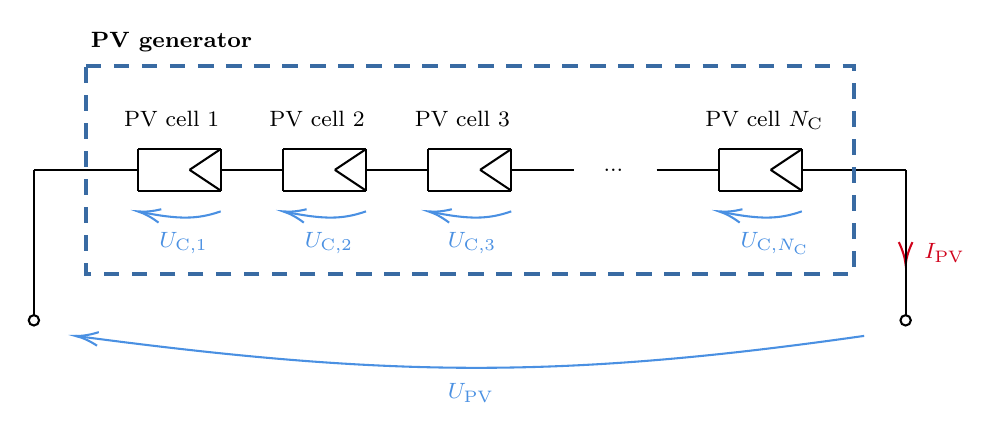
\begin{tikzpicture}[x=0.75pt,y=0.75pt,yscale=-1,xscale=1]
%uncomment if require: \path (0,300); %set diagram left start at 0, and has height of 300

%Straight Lines [id:da607551945482224] 
\draw [color={rgb, 255:red, 208; green, 2; blue, 27 }  ,draw opacity=1 ]   (560,180) -- (560,193.75) ;
\draw [shift={(560,195.75)}, rotate = 270] [color={rgb, 255:red, 208; green, 2; blue, 27 }  ,draw opacity=1 ][line width=0.75]    (10.93,-3.29) .. controls (6.95,-1.4) and (3.31,-0.3) .. (0,0) .. controls (3.31,0.3) and (6.95,1.4) .. (10.93,3.29)   ;
%Straight Lines [id:da39220891738716435] 
\draw    (370,140) -- (370,160) ;
%Straight Lines [id:da26376681003549773] 
\draw    (370,140) -- (355,150) ;
%Straight Lines [id:da7171194033958681] 
\draw    (355,150) -- (370,160) ;
%Straight Lines [id:da7758232590553849] 
\draw    (370,140) -- (330,140) ;
%Straight Lines [id:da23922780724985704] 
\draw    (370,160) -- (330,160) ;
%Straight Lines [id:da8647396746050291] 
\draw    (330,140) -- (330,160) ;
%Shape: Circle [id:dp9465717065223571] 
\draw   (560,220) .. controls (561.38,220) and (562.5,221.12) .. (562.5,222.5) .. controls (562.5,223.88) and (561.38,225) .. (560,225) .. controls (558.62,225) and (557.5,223.88) .. (557.5,222.5) .. controls (557.5,221.12) and (558.62,220) .. (560,220) -- cycle ;
%Straight Lines [id:da8361729954042678] 
\draw    (300,140) -- (300,160) ;
%Straight Lines [id:da8303503310697085] 
\draw    (300,140) -- (285,150) ;
%Straight Lines [id:da6935206293495084] 
\draw    (285,150) -- (300,160) ;
%Straight Lines [id:da4478328338561339] 
\draw    (300,140) -- (260,140) ;
%Straight Lines [id:da6338115192168345] 
\draw    (300,160) -- (260,160) ;
%Straight Lines [id:da4710313866121387] 
\draw    (260,140) -- (260,160) ;
%Straight Lines [id:da04529427678773623] 
\draw    (510,140) -- (510,160) ;
%Straight Lines [id:da12585917694032633] 
\draw    (510,140) -- (495,150) ;
%Straight Lines [id:da5777912998057524] 
\draw    (495,150) -- (510,160) ;
%Straight Lines [id:da8526647582658238] 
\draw    (510,140) -- (470,140) ;
%Straight Lines [id:da18181567227521733] 
\draw    (510,160) -- (470,160) ;
%Straight Lines [id:da08821152259447507] 
\draw    (470,140) -- (470,160) ;
%Straight Lines [id:da004318261204414364] 
\draw    (300,150) -- (330,150) ;
%Straight Lines [id:da415576466861697] 
\draw    (440,150) -- (470,150) ;
%Straight Lines [id:da5030082829613725] 
\draw    (230,140) -- (230,160) ;
%Straight Lines [id:da24153450583970604] 
\draw    (230,140) -- (215,150) ;
%Straight Lines [id:da7169826080141817] 
\draw    (215,150) -- (230,160) ;
%Straight Lines [id:da8893075482646204] 
\draw    (230,140) -- (190,140) ;
%Straight Lines [id:da8414185658377555] 
\draw    (230,160) -- (190,160) ;
%Straight Lines [id:da030501270201809483] 
\draw    (190,140) -- (190,160) ;
%Straight Lines [id:da11000547395248828] 
\draw    (140,150) -- (190,150) ;
%Straight Lines [id:da8573962154803463] 
\draw    (230,150) -- (260,150) ;
%Straight Lines [id:da9793828451968309] 
\draw    (370,150) -- (400,150) ;
%Straight Lines [id:da6281863128480734] 
\draw    (510,150) -- (560,150) ;
%Shape: Rectangle [id:dp583588773515656] 
\draw  [color={rgb, 255:red, 57; green, 107; blue, 163 }  ,draw opacity=1 ][dash pattern={on 5.63pt off 4.5pt}][line width=1.5]  (165,100) -- (535,100) -- (535,200) -- (165,200) -- cycle ;
%Curve Lines [id:da418839437477464] 
\draw [color={rgb, 255:red, 74; green, 144; blue, 226 }  ,draw opacity=1 ]   (230,170) .. controls (218.85,173.88) and (210.04,174) .. (191.73,170.35) ;
\draw [shift={(190,170)}, rotate = 371.59000000000003] [color={rgb, 255:red, 74; green, 144; blue, 226 }  ,draw opacity=1 ][line width=0.75]    (10.93,-3.29) .. controls (6.95,-1.4) and (3.31,-0.3) .. (0,0) .. controls (3.31,0.3) and (6.95,1.4) .. (10.93,3.29)   ;
%Curve Lines [id:da498717897550782] 
\draw [color={rgb, 255:red, 74; green, 144; blue, 226 }  ,draw opacity=1 ]   (300,170) .. controls (288.84,173.88) and (280.04,174) .. (261.73,170.35) ;
\draw [shift={(260,170)}, rotate = 371.59000000000003] [color={rgb, 255:red, 74; green, 144; blue, 226 }  ,draw opacity=1 ][line width=0.75]    (10.93,-3.29) .. controls (6.95,-1.4) and (3.31,-0.3) .. (0,0) .. controls (3.31,0.3) and (6.95,1.4) .. (10.93,3.29)   ;
%Curve Lines [id:da08475302030352005] 
\draw [color={rgb, 255:red, 74; green, 144; blue, 226 }  ,draw opacity=1 ]   (370,170) .. controls (358.85,173.88) and (350.04,174) .. (331.73,170.35) ;
\draw [shift={(330,170)}, rotate = 371.59000000000003] [color={rgb, 255:red, 74; green, 144; blue, 226 }  ,draw opacity=1 ][line width=0.75]    (10.93,-3.29) .. controls (6.95,-1.4) and (3.31,-0.3) .. (0,0) .. controls (3.31,0.3) and (6.95,1.4) .. (10.93,3.29)   ;
%Curve Lines [id:da12741622664998054] 
\draw [color={rgb, 255:red, 74; green, 144; blue, 226 }  ,draw opacity=1 ]   (510,170) .. controls (498.85,173.88) and (490.04,174) .. (471.73,170.35) ;
\draw [shift={(470,170)}, rotate = 371.59000000000003] [color={rgb, 255:red, 74; green, 144; blue, 226 }  ,draw opacity=1 ][line width=0.75]    (10.93,-3.29) .. controls (6.95,-1.4) and (3.31,-0.3) .. (0,0) .. controls (3.31,0.3) and (6.95,1.4) .. (10.93,3.29)   ;
%Straight Lines [id:da46920157249938654] 
\draw    (560,150) -- (560,220) ;
%Shape: Circle [id:dp649544243274581] 
\draw   (140,220) .. controls (141.38,220) and (142.5,221.12) .. (142.5,222.5) .. controls (142.5,223.88) and (141.38,225) .. (140,225) .. controls (138.62,225) and (137.5,223.88) .. (137.5,222.5) .. controls (137.5,221.12) and (138.62,220) .. (140,220) -- cycle ;
%Straight Lines [id:da23605717922255787] 
\draw    (140,150) -- (140,220) ;
%Curve Lines [id:da371666183196145] 
\draw [color={rgb, 255:red, 74; green, 144; blue, 226 }  ,draw opacity=1 ]   (540,230) .. controls (392.5,251) and (310.5,250) .. (160,230) ;
\draw [shift={(160,230)}, rotate = 367.57] [color={rgb, 255:red, 74; green, 144; blue, 226 }  ,draw opacity=1 ][line width=0.75]    (10.93,-3.29) .. controls (6.95,-1.4) and (3.31,-0.3) .. (0,0) .. controls (3.31,0.3) and (6.95,1.4) .. (10.93,3.29)   ;

% Text Node
\draw (182,120) node [anchor=north west][inner sep=0.75pt]  [font=\footnotesize] [align=left] {PV cell $\displaystyle 1$};
% Text Node
\draw (567.5,183.9) node [anchor=north west][inner sep=0.75pt]  [font=\footnotesize,color={rgb, 255:red, 208; green, 2; blue, 27 }  ,opacity=1 ]  {$I_{\mathrm{PV}}$};
% Text Node
\draw (199,178.4) node [anchor=north west][inner sep=0.75pt]  [font=\footnotesize,color={rgb, 255:red, 74; green, 144; blue, 226 }  ,opacity=1 ]  {$U_{\mathrm{C,} 1}$};
% Text Node
\draw (269,178.4) node [anchor=north west][inner sep=0.75pt]  [font=\footnotesize,color={rgb, 255:red, 74; green, 144; blue, 226 }  ,opacity=1 ]  {$U_{\mathrm{C} ,2}$};
% Text Node
\draw (338,178.4) node [anchor=north west][inner sep=0.75pt]  [font=\footnotesize,color={rgb, 255:red, 74; green, 144; blue, 226 }  ,opacity=1 ]  {$U_{\mathrm{C} ,3}$};
% Text Node
\draw (479,178.4) node [anchor=north west][inner sep=0.75pt]  [font=\footnotesize,color={rgb, 255:red, 74; green, 144; blue, 226 }  ,opacity=1 ]  {$U_{\mathrm{C} ,N_{\mathrm{C}}}$};
% Text Node
\draw (252,120) node [anchor=north west][inner sep=0.75pt]  [font=\footnotesize] [align=left] {PV cell $\displaystyle 2$};
% Text Node
\draw (322,120) node [anchor=north west][inner sep=0.75pt]  [font=\footnotesize] [align=left] {PV cell $\displaystyle 3$};
% Text Node
\draw (462,120) node [anchor=north west][inner sep=0.75pt]  [font=\footnotesize] [align=left] {PV cell $\displaystyle N_{\mathrm{C}}$};
% Text Node
\draw (338,251.4) node [anchor=north west][inner sep=0.75pt]  [font=\footnotesize,color={rgb, 255:red, 74; green, 144; blue, 226 }  ,opacity=1 ]  {$U_{\mathrm{PV}}$};
% Text Node
\draw (413,148) node [anchor=north west][inner sep=0.75pt]  [font=\footnotesize] [align=left] {...};
% Text Node
\draw (166,82) node [anchor=north west][inner sep=0.75pt]  [font=\footnotesize] [align=left] {\textbf{PV generator}};


\end{tikzpicture}

	\caption{Circuit diagram of a photovoltaic generator. It consists of $n = N_{\mathrm{PVC}}$ photovoltaic cells connected in series. (Recreated from: \cite{Mertens:2015})}
	\label{fig:tikz_PVG_circuit_diagram}
\end{figure}
It can be seen, that $I_{\mathrm{PVG}}$ is equal for all PVCs and that $U_{\mathrm{PVG}}$ is the sum of the \emph{PVC voltages} $U_{\mathrm{PVC}}$. In this thesis it is assumed that all PVCs have the same voltage $U_{\mathrm{PVC}}$, and therefore $U_{\mathrm{PVG}}$ can be written as presented in equation \ref{eq:u_pvg_sum_of_pvc}. For the sake of simplicity it is furthermore assumed, that the PVG is installed in a way, so that no shadowing occurs during the course of the mission \cite{Prechtl:2006, Mertens:2015}.

\begin{center}
	\begin{equation} \label{eq:u_pvg_sum_of_pvc}
		U_{\mathrm{PVG}} = N_{\mathrm{PVC}} \, U_{\mathrm{PVC}}
	\end{equation}
\end{center}

In the next step the PVCs shown in figure \ref{fig:tikz_PVG_circuit_diagram} must be modeled. For this, the simplified standard model\footnote{This model can be derived from the PVC standard model for $R_{\mathrm{P}} \to \infty$ and $R_{\mathrm{S}} = 0\Omega$.} is used, as there are explicit solutions for $U_{\mathrm{PVC}}$ and $I_{\mathrm{PVG}}$. It represents an ideal PVC without internal losses. An illustration of this model is provided in figure \ref{fig:tikz_PVC_simplified} \cite{Mertens:2015, Wagner:2018}.
\begin{figure}[h!]
	\centering
	

\tikzset{every picture/.style={line width=0.75pt}} %set default line width to 0.75pt        

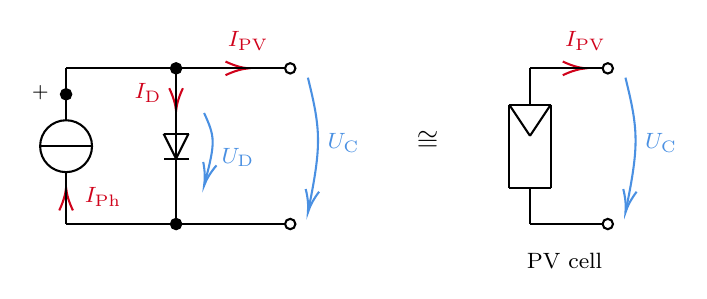
\begin{tikzpicture}[x=0.75pt,y=0.75pt,yscale=-1,xscale=1]
%uncomment if require: \path (0,391); %set diagram left start at 0, and has height of 391

%Straight Lines [id:da9220046892300695] 
\draw [color={rgb, 255:red, 208; green, 2; blue, 27 }  ,draw opacity=1 ]   (259.5,142.5) -- (273.25,142.5) ;
\draw [shift={(275.25,142.5)}, rotate = 180] [color={rgb, 255:red, 208; green, 2; blue, 27 }  ,draw opacity=1 ][line width=0.75]    (10.93,-3.29) .. controls (6.95,-1.4) and (3.31,-0.3) .. (0,0) .. controls (3.31,0.3) and (6.95,1.4) .. (10.93,3.29)   ;
%Straight Lines [id:da9695421868123493] 
\draw [color={rgb, 255:red, 208; green, 2; blue, 27 }  ,draw opacity=1 ]   (422,142.5) -- (435.75,142.5) ;
\draw [shift={(437.75,142.5)}, rotate = 180] [color={rgb, 255:red, 208; green, 2; blue, 27 }  ,draw opacity=1 ][line width=0.75]    (10.93,-3.29) .. controls (6.95,-1.4) and (3.31,-0.3) .. (0,0) .. controls (3.31,0.3) and (6.95,1.4) .. (10.93,3.29)   ;
%Straight Lines [id:da29339333794333666] 
\draw [color={rgb, 255:red, 208; green, 2; blue, 27 }  ,draw opacity=1 ]   (240.5,142.5) -- (240.5,161) ;
\draw [shift={(240.5,163)}, rotate = 270] [color={rgb, 255:red, 208; green, 2; blue, 27 }  ,draw opacity=1 ][line width=0.75]    (10.93,-3.29) .. controls (6.95,-1.4) and (3.31,-0.3) .. (0,0) .. controls (3.31,0.3) and (6.95,1.4) .. (10.93,3.29)   ;
%Straight Lines [id:da5182268392298646] 
\draw [color={rgb, 255:red, 208; green, 2; blue, 27 }  ,draw opacity=1 ]   (187.5,212.5) -- (187.5,202) ;
\draw [shift={(187.5,200)}, rotate = 450] [color={rgb, 255:red, 208; green, 2; blue, 27 }  ,draw opacity=1 ][line width=0.75]    (10.93,-3.29) .. controls (6.95,-1.4) and (3.31,-0.3) .. (0,0) .. controls (3.31,0.3) and (6.95,1.4) .. (10.93,3.29)   ;
%Straight Lines [id:da19579076658988703] 
\draw    (187.5,192.5) -- (187.5,217.5) ;
%Straight Lines [id:da500967170364542] 
\draw    (240.5,142.5) -- (240.5,217.5) ;
%Straight Lines [id:da9693092867247253] 
\draw    (187.5,142.5) -- (187.5,167.5) ;
%Straight Lines [id:da3180920793144646] 
\draw    (240.5,186) -- (234.5,186) ;
%Straight Lines [id:da3231236229149821] 
\draw    (246.5,186) -- (240.5,186) ;
%Straight Lines [id:da20274569848223778] 
\draw    (246.5,174) -- (240.5,174) ;
%Straight Lines [id:da4237476648515044] 
\draw    (240.5,174) -- (234.5,174) ;
%Straight Lines [id:da7091520922682297] 
\draw    (234.5,174) -- (240.5,186) ;
%Straight Lines [id:da8216387087718504] 
\draw    (240.5,186) -- (246.5,174) ;
%Shape: Circle [id:dp46632786849059626] 
\draw   (175,180) .. controls (175,173.1) and (180.6,167.5) .. (187.5,167.5) .. controls (194.4,167.5) and (200,173.1) .. (200,180) .. controls (200,186.9) and (194.4,192.5) .. (187.5,192.5) .. controls (180.6,192.5) and (175,186.9) .. (175,180) -- cycle ;
%Straight Lines [id:da6428722008154575] 
\draw    (175,180) -- (200,180) ;
%Shape: Circle [id:dp9143776877359857] 
\draw  [fill={rgb, 255:red, 0; green, 0; blue, 0 }  ,fill opacity=1 ] (238,217.5) .. controls (238,216.12) and (239.12,215) .. (240.5,215) .. controls (241.88,215) and (243,216.12) .. (243,217.5) .. controls (243,218.88) and (241.88,220) .. (240.5,220) .. controls (239.12,220) and (238,218.88) .. (238,217.5) -- cycle ;
%Shape: Circle [id:dp04116434903611532] 
\draw  [fill={rgb, 255:red, 0; green, 0; blue, 0 }  ,fill opacity=1 ] (185,155) .. controls (185,153.62) and (186.12,152.5) .. (187.5,152.5) .. controls (188.88,152.5) and (190,153.62) .. (190,155) .. controls (190,156.38) and (188.88,157.5) .. (187.5,157.5) .. controls (186.12,157.5) and (185,156.38) .. (185,155) -- cycle ;
%Shape: Circle [id:dp7561083964816784] 
\draw  [fill={rgb, 255:red, 0; green, 0; blue, 0 }  ,fill opacity=1 ] (238,142.5) .. controls (238,141.12) and (239.12,140) .. (240.5,140) .. controls (241.88,140) and (243,141.12) .. (243,142.5) .. controls (243,143.88) and (241.88,145) .. (240.5,145) .. controls (239.12,145) and (238,143.88) .. (238,142.5) -- cycle ;
%Curve Lines [id:da12939293693438314] 
\draw [color={rgb, 255:red, 74; green, 144; blue, 226 }  ,draw opacity=1 ]   (254,164) .. controls (259.33,175.64) and (259.5,177.87) .. (254.48,197.16) ;
\draw [shift={(254,199)}, rotate = 284.68] [color={rgb, 255:red, 74; green, 144; blue, 226 }  ,draw opacity=1 ][line width=0.75]    (10.93,-3.29) .. controls (6.95,-1.4) and (3.31,-0.3) .. (0,0) .. controls (3.31,0.3) and (6.95,1.4) .. (10.93,3.29)   ;
%Straight Lines [id:da820440930056753] 
\draw    (401,160) -- (421,160) ;
%Straight Lines [id:da5978422659023195] 
\draw    (401,160) -- (411,175) ;
%Straight Lines [id:da8646077617642114] 
\draw    (411,175) -- (421,160) ;
%Straight Lines [id:da1683854382748906] 
\draw    (401,160) -- (401,200) ;
%Straight Lines [id:da35944219412656886] 
\draw    (421,160) -- (421,200) ;
%Straight Lines [id:da012841517263090685] 
\draw    (401,200) -- (421,200) ;
%Straight Lines [id:da8937999883743217] 
\draw    (411,200) -- (411,217.5) ;
%Shape: Circle [id:dp39581519495881] 
\draw   (446,142.5) .. controls (446,141.12) and (447.12,140) .. (448.5,140) .. controls (449.88,140) and (451,141.12) .. (451,142.5) .. controls (451,143.88) and (449.88,145) .. (448.5,145) .. controls (447.12,145) and (446,143.88) .. (446,142.5) -- cycle ;
%Shape: Circle [id:dp7404102366707606] 
\draw   (446,217.5) .. controls (446,216.12) and (447.12,215) .. (448.5,215) .. controls (449.88,215) and (451,216.12) .. (451,217.5) .. controls (451,218.88) and (449.88,220) .. (448.5,220) .. controls (447.12,220) and (446,218.88) .. (446,217.5) -- cycle ;
%Straight Lines [id:da16056380159184358] 
\draw    (411,142.5) -- (446,142.5) ;
%Straight Lines [id:da8365114488683654] 
\draw    (411,217.5) -- (446,217.5) ;
%Curve Lines [id:da5511080558248806] 
\draw [color={rgb, 255:red, 74; green, 144; blue, 226 }  ,draw opacity=1 ]   (457,147) .. controls (463.37,172.48) and (463.5,179.71) .. (457.38,210.11) ;
\draw [shift={(457,212)}, rotate = 281.48] [color={rgb, 255:red, 74; green, 144; blue, 226 }  ,draw opacity=1 ][line width=0.75]    (10.93,-3.29) .. controls (6.95,-1.4) and (3.31,-0.3) .. (0,0) .. controls (3.31,0.3) and (6.95,1.4) .. (10.93,3.29)   ;
%Straight Lines [id:da725857721119765] 
\draw    (411,142.5) -- (411,160) ;
%Straight Lines [id:da5740090703572132] 
\draw    (187.5,142.5) -- (240.5,142.5) ;
%Straight Lines [id:da4778393661136311] 
\draw    (187.5,217.5) -- (240.5,217.5) ;
%Shape: Circle [id:dp2917985814178987] 
\draw   (293,142.5) .. controls (293,141.12) and (294.12,140) .. (295.5,140) .. controls (296.88,140) and (298,141.12) .. (298,142.5) .. controls (298,143.88) and (296.88,145) .. (295.5,145) .. controls (294.12,145) and (293,143.88) .. (293,142.5) -- cycle ;
%Shape: Circle [id:dp07126668235633615] 
\draw   (293,217.5) .. controls (293,216.12) and (294.12,215) .. (295.5,215) .. controls (296.88,215) and (298,216.12) .. (298,217.5) .. controls (298,218.88) and (296.88,220) .. (295.5,220) .. controls (294.12,220) and (293,218.88) .. (293,217.5) -- cycle ;
%Curve Lines [id:da8740596681425179] 
\draw [color={rgb, 255:red, 74; green, 144; blue, 226 }  ,draw opacity=1 ]   (304,147) .. controls (310.37,172.48) and (310.5,179.71) .. (304.38,210.11) ;
\draw [shift={(304,212)}, rotate = 281.48] [color={rgb, 255:red, 74; green, 144; blue, 226 }  ,draw opacity=1 ][line width=0.75]    (10.93,-3.29) .. controls (6.95,-1.4) and (3.31,-0.3) .. (0,0) .. controls (3.31,0.3) and (6.95,1.4) .. (10.93,3.29)   ;
%Straight Lines [id:da2745454915751546] 
\draw    (240.5,142.5) -- (293.5,142.5) ;
%Straight Lines [id:da3914094245668047] 
\draw    (240.5,217.5) -- (293.5,217.5) ;

% Text Node
\draw (219,148.4) node [anchor=north west][inner sep=0.75pt]  [font=\footnotesize,color={rgb, 255:red, 208; green, 2; blue, 27 }  ,opacity=1 ]  {$I_{\mathrm{D}}$};
% Text Node
\draw (195,198.4) node [anchor=north west][inner sep=0.75pt]  [font=\footnotesize,color={rgb, 255:red, 208; green, 2; blue, 27 }  ,opacity=1 ]  {$I_{\mathrm{Ph}}$};
% Text Node
\draw (261,179.4) node [anchor=north west][inner sep=0.75pt]  [font=\footnotesize,color={rgb, 255:red, 74; green, 144; blue, 226 }  ,opacity=1 ]  {$U_{\mathrm{D}}$};
% Text Node
\draw (355,171.4) node [anchor=north west][inner sep=0.75pt]  [font=\normalsize]  {$\cong $};
% Text Node
\draw (465,172.4) node [anchor=north west][inner sep=0.75pt]  [font=\footnotesize,color={rgb, 255:red, 74; green, 144; blue, 226 }  ,opacity=1 ]  {$U_{\mathrm{C}}$};
% Text Node
\draw (426.5,123.4) node [anchor=north west][inner sep=0.75pt]  [font=\footnotesize,color={rgb, 255:red, 208; green, 2; blue, 27 }  ,opacity=1 ]  {$I_{\mathrm{PV}}$};
% Text Node
\draw (408,230) node [anchor=north west][inner sep=0.75pt]  [font=\footnotesize] [align=left] {PV cell};
% Text Node
\draw (312,172.4) node [anchor=north west][inner sep=0.75pt]  [font=\footnotesize,color={rgb, 255:red, 74; green, 144; blue, 226 }  ,opacity=1 ]  {$U_{\mathrm{C}}$};
% Text Node
\draw (264,123.4) node [anchor=north west][inner sep=0.75pt]  [font=\footnotesize,color={rgb, 255:red, 208; green, 2; blue, 27 }  ,opacity=1 ]  {$I_{\mathrm{PV}}$};
% Text Node
\draw (169.5,149.4) node [anchor=north west][inner sep=0.75pt]  [font=\scriptsize]  {$+$};


\end{tikzpicture}

	\caption{Simplified standard model of a photovoltaic cell. (Recreated from: \cite{Mertens:2015, Wagner:2018})}
	\label{fig:tikz_PVC_simplified}
\end{figure}

After applying Kirchoff's first and second law to the simplified standard model, considering equation \ref{eq:u_pvg_sum_of_pvc}, and taking into account that the PVG's current-voltage characteristic depends on the \emph{PVC temperature} $\vartheta = \vartheta_{\mathrm{PVC}}$ and the -- already introduced -- radiation flux $\Phi = \Phi_{\mathrm{GEN}}$, it can be modeled with the equations \ref{eq:i_of_u} and \ref{eq:u_of_i}.\footnote{Eqaution \ref{eq:u_of_i} can be derived from equations \ref{eq:i_of_u}.}
\begin{center}
	\begin{equation} \label{eq:i_of_u}
		I_{\mathrm{PVG}}\left(U_{\mathrm{PVG}}, \vartheta, \Phi\right) = I_{\mathrm{Ph}} - \underbrace{I_{\mathrm{S}} \left( \exp \left(\frac{U_{\mathrm{PVG}}}{m \, N_{\mathrm{PVC}} \, U_{\mathrm{T}} } \right) - 1  \right)}_{I_{\mathrm{D}}}
	\end{equation}
\end{center}
\begin{center}
	\begin{equation} \label{eq:u_of_i}
		U_{\mathrm{PVG}}\left(I_{\mathrm{PVG}}, \vartheta, \Phi\right) = m \, N_{\mathrm{PVC}} \, U_{\mathrm{T}} \, \ln \left( \frac{I_{\mathrm{Ph}} - I_{\mathrm{PVG}} + I_{\mathrm{S}}}{I_{\mathrm{S}}} \right)
	\end{equation}
\end{center}
The diode's \emph{thermal voltage} $U_{\mathrm{T}} = U_{\mathrm{T}}\left( \vartheta \right)$, with $k = 1,380649 \cdot 10^{-23} \mathrm{Ws/K}$ being the \emph{Bolzmann constant} and $e = 1,602176634\cdot10^{-19} \mathrm{As}$ being the \emph{elementary charge}, can be obtained from equation \ref{eq:u_temp}.
\begin{center}
	\begin{equation} \label{eq:u_temp}
		U_{\mathrm{T}}\left( \vartheta \right) = \frac{ k \, \left( \vartheta_{\mathrm{PVC}} + 273,15^\circ \mathrm{C} \right) }{e} \cdot \frac{\mathrm{1K}}{1^\circ \mathrm{C}}
	\end{equation}
\end{center}
$m$ is the \emph{ideality factor} with the condition $\{m \in \mathbb{R}^+ \mid 2 \geq m \geq 1 \}$. It is an empirical value that is used to model the PVCs more precisely.\footnote{For $m = 1$, $I_\mathrm{D}$ is Shockley's equation.} And the quantities $I_{\mathrm{S}} = I_{\mathrm{S}}\left( \vartheta \right)$ and $I_{\mathrm{Ph}} = I_{\mathrm{Ph}}\left(\vartheta, \Phi\right)$ are the diode's \emph{reverse saturation current} and the PVC's \emph{photocurrent}. How the PVC temperature $\vartheta_{\mathrm{PVC}}$ is determined will be explained later \cite{Prechtl:2006, Mertens:2015, Tietze:2016, Wagner:2018, Elert:2020}. 

Based on equation \ref{eq:i_of_u} the modeled current-voltage characteristic can be visualized as shown in figure \ref{fig:tikz/tikz_PVG_curve}, where $I_{\mathrm{SC}}\left(\vartheta,\Phi\right)$ and $U_{\mathrm{OC}}\left(\vartheta,\Phi\right)$ are the PVG's \emph{short-circuit current} and \emph{open-circuit voltage}. The MPP is the \emph{maximum power point}, for which the PVG provides the greatest electrical power \cite{Prechtl:2006, Mertens:2015, Wagner:2018}:
\begin{center}
	\begin{equation} \label{eq:p_mpp}
		P_{\mathrm{MPP}} = U_{\mathrm{MPP}} \, I_{\mathrm{MPP}} \text{.}
	\end{equation}
\end{center}
\begin{figure}[h!]
	\centering
	

\tikzset{every picture/.style={line width=0.75pt}} %set default line width to 0.75pt        

\begin{tikzpicture}[x=0.75pt,y=0.75pt,yscale=-1,xscale=1]
%uncomment if require: \path (0,300); %set diagram left start at 0, and has height of 300

%Image [id:dp8816301757772553] 
\draw (309.25,160) node [xscale=-1] {\includegraphics[width=211.13pt,height=180pt]{images/image_PVC_curve}};
%Straight Lines [id:da8531224351110531] 
\draw [color={rgb, 255:red, 155; green, 155; blue, 155 }  ,draw opacity=1 ] [dash pattern={on 4.5pt off 4.5pt}]  (184,113) -- (358,113) ;
%Straight Lines [id:da1728021335997585] 
\draw [color={rgb, 255:red, 155; green, 155; blue, 155 }  ,draw opacity=1 ] [dash pattern={on 4.5pt off 4.5pt}]  (358,113) -- (358,269) ;
%Shape: Circle [id:dp9850794530438081] 
\draw  [fill={rgb, 255:red, 255; green, 255; blue, 255 }  ,fill opacity=1 ] (356,113) .. controls (356,111.9) and (356.9,111) .. (358,111) .. controls (359.1,111) and (360,111.9) .. (360,113) .. controls (360,114.1) and (359.1,115) .. (358,115) .. controls (356.9,115) and (356,114.1) .. (356,113) -- cycle ;

% Text Node
\draw (129,19.4) node [anchor=north west][inner sep=0.75pt]  [font=\footnotesize]  {$I_{\mathrm{PV}}( U_{\mathrm{PV}} ,\vartheta _{\mathrm{C}} ,\Phi _{\mathrm{G}})$};
% Text Node
\draw (456,263.4) node [anchor=north west][inner sep=0.75pt]  [font=\footnotesize]  {$U_{\mathrm{PV}}$};
% Text Node
\draw (278,276.4) node [anchor=north west][inner sep=0.75pt]  [font=\footnotesize]  {$U_{\mathrm{MPP}}( \vartheta _{\mathrm{C}} ,\Phi _{\mathrm{G}})$};
% Text Node
\draw (91,105.4) node [anchor=north west][inner sep=0.75pt]  [font=\footnotesize]  {$I_{\mathrm{MPP}}( \vartheta _{\mathrm{C}} ,\Phi _{\mathrm{G}})$};
% Text Node
\draw (361,96) node [anchor=north west][inner sep=0.75pt]  [font=\footnotesize] [align=left] {MPP};
% Text Node
\draw (370,276.4) node [anchor=north west][inner sep=0.75pt]  [font=\footnotesize]  {$U_{\mathrm{OC}}( \vartheta _{\mathrm{C}} ,\Phi _{\mathrm{G}})$};
% Text Node
\draw (102,83.4) node [anchor=north west][inner sep=0.75pt]  [font=\footnotesize]  {$I_{\mathrm{SC}}( \vartheta _{\mathrm{C}} ,\Phi _{\mathrm{G}})$};
% Text Node
\draw (166,273.4) node [anchor=north west][inner sep=0.75pt]  [font=\footnotesize]  {$0$};


\end{tikzpicture}


	\caption{Modeled current-voltage characteristic of a photovoltaic generator depending on the radiation flux $\Phi = \Phi_{\mathrm{GEN}}$ and the photovoltaic cell temperature $\vartheta = \vartheta_{\mathrm{PVC}}$. (Recreated from: \cite{Mertens:2015, Wagner:2018})}
	\label{fig:tikz/tikz_PVG_curve}
\end{figure}

The quantity in the simplified standard model that changes with the solar radiation, is the photocurrent. It is proportional to the radiation flux $\Phi_{\mathrm{GEN}}$, with $S = \mathrm{const.}$ being the \emph{sensitivity} of the PVC:
\begin{center}
	\begin{equation} \label{eq:photo_i}
		I_{\mathrm{Ph}}\left( \vartheta_{\mathrm{STC}}, \Phi \right) = S \, \Phi_{\mathrm{GEN}} \text{.}
	\end{equation}
\end{center}
In the case $I_{\mathrm{PVG}}\left(0\mathrm{V}, \vartheta_{\mathrm{STC}}, \Phi_{\mathrm{STC}}\right) = I_\mathrm{SC,STC}$ the sensitivity results from equation \ref{eq:sens}.
\begin{center}
	\begin{equation} \label{eq:sens}
		 S = \frac{I_\mathrm{SC,STC}}{\Phi_{\mathrm{STC}}}
	\end{equation}
\end{center}
For the standard test conditions (STC), listed in table \ref{tab:table_STC}, $I_\mathrm{SC,STC}$ can be taken directly from the data sheet of the PVG and $\Phi_{\mathrm{STC}}$ can be obtained from equation \ref{eq:radiation_flux}. In this, $A_\mathrm{PVG}$ can either be measured or taken from the PVG's data sheet as well.
\begin{table}[h!]
	\centering
	\footnotesize
\begin{tabular}{|l|c|}
	\hline
	\multicolumn{2}{|c|}{\textbf{Standard test conditions for PV generators}} \\
	\hline
 	Total irradiance received by the PV generator & $E_{\mathrm{STC}} = 1000\mathrm{W} \mathrm{m}^{-2}$ \\
	PV cell temperature & $\vartheta_{\mathrm{STC}} = 25^\circ \mathrm{C}$ \\
	Solar spectrum & AM 1,5 \\
	\hline
\end{tabular}
	\caption{Parameters for the standard test conditions of a photovoltaic generator \cite{Mertens:2015}.}
	\label{tab:table_STC}
\end{table}
And finally, after substituting equation \ref{eq:sens} into equation \ref{eq:photo_i} and taking the \emph{temperature coefficient} of the short circuit current $\mathrm{TC}\left(I_{\mathrm{SC}}\right)$ into account, the photocurrent, depending on the PVC temperature and the radiation flux, follows to:
\begin{center}
	\begin{equation} \label{eq:i_ph_theta_phi}
		 I_{\mathrm{Ph}}\left( \vartheta, \Phi \right) = \underbrace{I_{\mathrm{SC,STC}} \, \frac{E_\mathrm{GEN}}{E_\mathrm{STC}}}_{I_{\mathrm{Ph}}\left( \vartheta_{\mathrm{STC}}, \Phi \right)} \, \left[ 1 + \frac{\mathrm{TC}\left(I_{\mathrm{SC}}\right)}{100\%} \left(\vartheta_{\mathrm{PVC}} - \vartheta_{\mathrm{STC}} \right) \right] \text{.}
	\end{equation}
\end{center}
$\mathrm{TC}\left(I_{\mathrm{SC}}\right)$ can usually be taken from the PVG's data sheet.\footnote{Typical $\mathrm{TC}\left(I_{\mathrm{SC}}\right)$ values for Si-PVCs are around $0,06 \% / \mathrm{K}$.} And because $I_{\mathrm{PVG}}\left( 0\mathrm{V}, \vartheta, \Phi \right) = I_{\mathrm{SC}}\left( \vartheta, \Phi \right)$, it follows, that $I_{\mathrm{SC}}\left( \vartheta, \Phi \right) = I_{\mathrm{Ph}}\left( \vartheta, \Phi \right)$ \cite{Mertens:2015, Tietze:2016, Wagner:2018}. 

Now that $I_{\mathrm{Ph}}\left( \vartheta, \Phi \right)$ is known, the diode's reverse saturation current can be calculated from the case $I_{\mathrm{PVG}}\left(U_{\mathrm{OC}}\left( \vartheta, \Phi \right), \vartheta, \Phi\right) = 0\mathrm{A}$: 
\begin{center}
	\begin{equation} \label{I_S_theta_phi}
		I_\mathrm{S}\left(\vartheta\right) = I_{\mathrm{Ph}}\left( \vartheta, \Phi \right) \, \left( \exp \left( \frac{U_\mathrm{OC}\left(\vartheta,\Phi\right)}{m \, N_\mathrm{PVC} \, U_\mathrm{T}} \right) - 1 \right)^{-1} \text{.}
	\end{equation}
\end{center}
The open-circuit voltage $U_\mathrm{OC}\left(\vartheta,\Phi\right)$ can be obtined by subtracting the case $U_{\mathrm{PVG}}\left( 0\mathrm{A}, \vartheta, \Phi \right)$ from the case $U_{\mathrm{PVG}}\left(0\mathrm{A}, \vartheta, \Phi_{\mathrm{STC}}\right)$, while taking the temperature coefficient of the open-circuit voltage $\mathrm{TC}\left(U_{\mathrm{OC}}\right)$ into account:
\begin{center}
	\begin{equation} \label{U_OC_theta_phi}
		U_\mathrm{OC}\left(\vartheta,\Phi\right) = U_\mathrm{OC}\left(\vartheta,\Phi_\mathrm{STC}\right)  + m \, N_\mathrm{PVC} \, U_\mathrm{T} \, \ln \left( \frac{I_{\mathrm{Ph}}\left(\vartheta, \Phi \right) + I_{\mathrm{S}}\left( \vartheta\right)}{I_\mathrm{Ph}\left(\vartheta,\Phi_\mathrm{STC}\right) + I_{\mathrm{S}}\left( \vartheta\right)} \right) \text{,}
	\end{equation}
\end{center}
where $U_\mathrm{OC}\left(\vartheta,\Phi_\mathrm{STC}\right)$ is the temperature depndent open-circuit voltage for the radiation flux $\Phi_\mathrm{STC}$ at STC: 
\begin{center}
	\begin{equation} \label{U_OC_phi_STC}
		U_\mathrm{OC}\left(\vartheta,\Phi_\mathrm{STC}\right) = U_\mathrm{OC,STC} \left[ 1 + \frac{\mathrm{TC}\left(U_{\mathrm{OC}}\right)}{100\%} \left(\vartheta_{\mathrm{PVC}} - \vartheta_{\mathrm{STC}} \right) \right] \text{.}
	\end{equation}
\end{center}
In addition to $\mathrm{TC}\left(I_{\mathrm{SC}}\right)$, $\mathrm{TC}\left(U_{\mathrm{OC}}\right)$ can also be taken from the PVG's data sheet.\footnote{Typical $\mathrm{TC}\left(U_{\mathrm{OC}}\right)$ values for Si-PVCs are around $-0,40 \% / ^\circ \mathrm{C}$.} Equation \ref{U_OC_theta_phi} is only valid becuase the reverse saturation current $I_\mathrm{S}\left(\vartheta\right)$ does not depend on the radiation flux \cite{Mertens:2015, Tietze:2016, Hering:2017, Wagner:2018}. 

Since both functions -- from the equations \ref{I_S_theta_phi} and \ref{U_OC_theta_phi} -- are in a non-linear relationship to one another, the Newton-Raphson method must be used to approximate them numerically (see appendix \ref{sec:newton_raphson_method}). For this, the functions $f_1\left( \mathrm{\mathbf{x}}_R \right)$ and $f_2\left( \mathrm{\mathbf{x}}_R \right)$ are introduced in the equations \ref{f_1} and \ref{f_2}. In first equation (\ref{f_1}) an exponential function is used instead of a logarthmic function, because some numerical approximation algorithms do not converge for logarithmic functions.
\begin{center}
	\begin{equation} \label{f_1}
		f_1 \left( \mathrm{\mathbf{x}}_R \right)  = \exp \left( \frac{U_\mathrm{OC}\left(\vartheta,\Phi\right) - U_\mathrm{OC}\left(\vartheta,\Phi_\mathrm{STC}\right)}{m \, N_\mathrm{PVC} \, U_\mathrm{T}} \right) - \frac{I_\mathrm{Ph}\left(\vartheta,\Phi\right) + I_\mathrm{S}\left(\vartheta\right)}{I_\mathrm{Ph}\left(\vartheta,\Phi_\mathrm{STC}\right) + I_\mathrm{S}\left(\vartheta\right)} = 0
	\end{equation}
\end{center}
\begin{center}
	\begin{equation} \label{f_2}
		f_2\left( \mathrm{\mathbf{x}}_R \right) = I_\mathrm{S}\left(\vartheta\right) - I_\mathrm{Ph}\left(\vartheta,\Phi\right) \, \left( \exp \left( \frac{U_\mathrm{OC}\left(\vartheta,\Phi\right)}{m \, N_\mathrm{PVC} \, U_\mathrm{T}} \right) - 1 \right)^{-1} = 0\mathrm{A}
	\end{equation}
\end{center}
The vector $\mathrm{\mathbf{x}}_R$ containes the zero crossings of the functions $f_1\left( \mathrm{\mathbf{x}}_R \right)$ and $f_2\left( \mathrm{\mathbf{x}}_R \right)$. It can be seen in equation \ref{x_r_vector}. 
\begin{center}
	\begin{equation} \label{x_r_vector}
		\mathrm{\mathbf{x}}_R = \Big( I_\mathrm{S}\left(\vartheta\right), U_\mathrm{OC}\left(\vartheta,\Phi\right) \Big)^{\mathrm T}
	\end{equation}
\end{center}
Furthermore, the vector $\mathrm{\mathbf{f}}\left(\mathrm{\mathbf{x}}_R\right) = \mathbf{0}$, which containes the functions from the equations \ref{f_1} and \ref{f_2}, must be introduced for the Newton-Raphson method:
\begin{center}
	\begin{equation} \label{f_vector}
		\mathrm{\mathbf{f}}\left(\mathrm{\mathbf{x}}_R\right) = 
  			\Big( f_{1} \left( \mathrm{\mathbf{x}}_R \right), f_{1} \left( \mathrm{\mathbf{x}}_R \right) \Big)^{\mathrm T} = \mathrm{\mathbf{0}} \text{.}
	\end{equation}
\end{center}
With the help of the Jacobian matrix $\mathrm{\mathbf{J}}$, the $\left(n + 1\right)$\textsuperscript{th} approximation with $n \in \mathbb{N}$, can be determined as follows:
\begin{center}
	\begin{equation} \label{eq:vect_U_I_approx}
		\mathrm{\mathbf{x}}_{R, n + 1} = \mathrm{\mathbf{x}}_{R,n} 	- \mathrm{\mathbf{J}}^{-1}\left( \mathrm{\mathbf{x}}_{R,n} \right) \, \mathrm{\mathbf{f}}\left( \mathrm{\mathbf{x}}_{R,n} \right) \text{,}
	\end{equation}
\end{center}
\begin{center}
	\begin{equation} \label{eq:jacobian_for_PVG}
		\mathrm{\mathbf{J}} = \left. \dfrac{\partial \mathrm{\mathbf{f}}\left(\mathrm{\mathbf{x}}\right)}{\partial \mathrm{\mathbf{x}}} \right|_{\mathrm{\mathbf{x}} = \mathrm{\mathbf{x}}_R} = 
 		\begin{pmatrix}
  			\dfrac{\partial f_1\big( I_\mathrm{S}\left(\vartheta\right), U_\mathrm{OC}\left(\vartheta,\Phi\right) \big)}{\partial I_\mathrm{S}\left(\vartheta\right)}  & \dfrac{\partial  f_1\big( I_\mathrm{S}\left(\vartheta\right), U_\mathrm{OC}\left(\vartheta,\Phi\right) \big)}{\partial U_\mathrm{OC}\left(\vartheta,\Phi\right)} \\
			\dfrac{\partial f_2\big( I_\mathrm{S}\left(\vartheta\right), U_\mathrm{OC}\left(\vartheta,\Phi\right) \big)}{\partial I_\mathrm{S}\left(\vartheta\right)} & \dfrac{\partial f_2\big( I_\mathrm{S}\left(\vartheta\right), U_\mathrm{OC}\left(\vartheta,\Phi\right) \big)}{\partial U_\mathrm{OC}\left(\vartheta,\Phi\right)} 
 		\end{pmatrix} \text{.}
 	\end{equation}
\end{center}
Starting values for the Newton-Raphson method can be obtained from the equtaions \ref{eq:U_OC_theta_phi_zero} and \ref{I_S_theta_phi_zero} if it is accepted, that the diode's reverse saturation current $I_{\mathrm{S}}$ is small compared to the photocurrent $I_{\mathrm{Ph}}$, so that $I_{\mathrm{S}} + I_{\mathrm{Ph}} \approx I_{\mathrm{Ph}}$ applies.\footnote{Equation \ref{eq:U_OC_theta_phi_zero} can be derived from equation \ref{eq:U_OC_theta_phi} and equation \ref{I_S_theta_phi_zero} can be derived from equation \ref{I_S_theta_phi}.}
\begin{center}
	\begin{equation} \label{eq:U_OC_theta_phi_zero}
		\begin{gathered}
		 U_{\mathrm{OC,0}}\left( \vartheta, \Phi \right) = U_\mathrm{OC}\left(\vartheta,\Phi_\mathrm{STC}\right) + m \, N_\mathrm{PVC} \, U_\mathrm{T} \, \ln \left( \frac{I_\mathrm{Ph}\left(\vartheta,\Phi\right)}{I_\mathrm{Ph}\left(\vartheta,\Phi_\mathrm{STC}\right)} \right) \text{,} \\ \text{for } I_\mathrm{S} \ll I_\mathrm{Ph}
		 \end{gathered}
	\end{equation}
\end{center}
\begin{center}
	\begin{equation} \label{I_S_theta_phi_zero}
		I_\mathrm{S,0}\left(\vartheta\right) = I_{\mathrm{Ph}}\left( \vartheta, \Phi \right) \, \exp \left( - \frac{U_\mathrm{OC}\left(\vartheta,\Phi\right)}{m \, N_\mathrm{PVC} \, U_\mathrm{T}} \right) \text{,} \quad \text{for } I_\mathrm{S} \ll I_\mathrm{Ph}
	\end{equation}
\end{center}
From these, the starting vector $\mathrm{\mathbf{x}}_{R,0} = \big( I_\mathrm{S,0}\left(\vartheta\right), U_\mathrm{OC,0}\left(\vartheta,\Phi\right) \big)^{\mathrm T}$ for the first iteration can determined. Finally it has to mentioned, that the functions $f_1\left( \mathrm{\mathbf{x}}_R \right)$ and $f_2\left( \mathrm{\mathbf{x}}_R \right)$ are continuously differentiable for the required number of iteration steps $n + 1$, which is a requirement of the Newton-Raphson method \cite{Schwarz:2011, Rudolf:2014, Taschner:2014, Mertens:2015, Wagner:2018, Kugi:2021}.

The PVC temperature $\vartheta_{\mathrm{PVC}}$, depending on the total irradiance $E_{\mathrm{GEN}}$ and the \emph{ambient temperature} $\vartheta_{\mathrm{A}}$, with the \emph{nominal operating cell temperature}\footnote{Typical $\mathrm{NOCT}$ values for c-Si-PVGs are around $45$ to $50^\circ \mathrm{C}$.} $\mathrm{NOCT}$ and the conditions under which it is measured, $\vartheta_{\mathrm{A,NOCT}}$ and $E_{\mathrm{NOCT}}$, can be approximated by assuming that the increase of $\vartheta_{\mathrm{PVC}}$, compared to the ambient temperature $\vartheta_{\mathrm{A}}$, is proportional to $E_{\mathrm{GEN}}$:
\begin{center}
	\begin{equation} \label{eq:cell_temp}
		\vartheta_{\mathrm{PVC}} \approx \vartheta_{\mathrm{A}} + \left(\mathrm{NOCT} - \vartheta_{\mathrm{A,NOCT}}\right) \frac{E_{\mathrm{GEN}}}{E_{\mathrm{NOCT}}} \text{.}
	\end{equation}
\end{center}
The paramateres under which the $\mathrm{NOCT}$ is measured are provided by table \ref{tab:table_NOCT} and the $\mathrm{NOCT}$ is usually listed in the PVG's data sheet as well \cite{Mertens:2015}.

\begin{table}[h!]
	\centering
	\footnotesize
\begin{tabular}{|l|c|}
	\hline
	\multicolumn{2}{|c|}{\textbf{Conditions for NOCT measurement}} \\
	\hline
 	Total irradiance received by the PV generator & $E_{\mathrm{NOCT}} = 800\mathrm{W} \mathrm{m}^{-2}$ \\
	Ambient temperature & $\vartheta_{\mathrm{A, NOCT}} = 20^\circ \mathrm{C}$ \\
	Wind speed & $v_{\mathrm W} = 1 \mathrm{m} \mathrm{s}^{-1}$  \\
	\hline
\end{tabular}
	\caption{Conditions under which the NOCT is measured \cite{Mertens:2015}.}
	\label{tab:table_NOCT}
\end{table}

Ambient temperatures $\vartheta_{\mathrm{A}}$ for different locations on Earth can be obtained from climate charts. Figure \ref{fig:temp_vienna}, for example, presents monthly averages for the ambient temperature in $^\circ \mathrm{C}$ and precipitation in $\mathrm{mm}$, collected by the Global Historical Climatology Network, for the Hohe Warte in Vienna, Austria, between 1997 and 2016. Below the chart the percentage of missing data, regarding the months of the year, is presented. More climate charts can be found in appendix \ref{ap:solar_resource_maps} \cite{Zepner:2020}.

\begin{figure}[h!]
	\centering
  	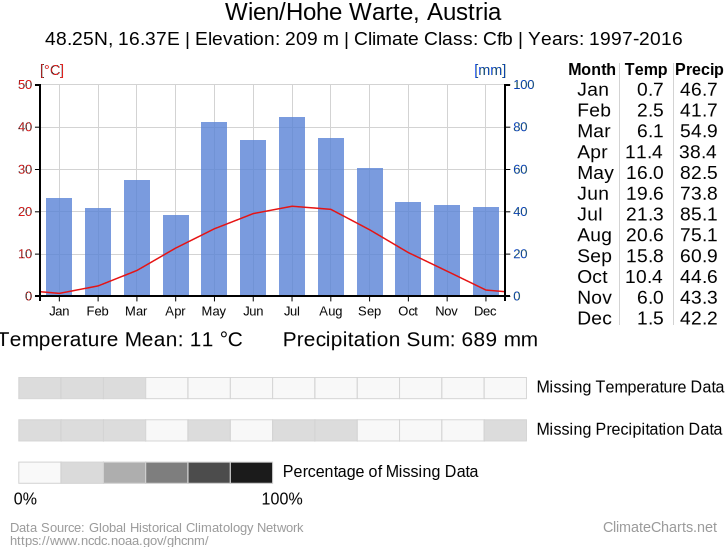
\includegraphics[width = 0.96\textwidth]{temp_maps/temp_vienna}
  	\caption{Monthly averages of temperature and precipitation data for the Hohe Warte in Vienna, Austria. (Image credit: \cite{Zepner:2020} and \emph{climatecharts.net})}
	\label{fig:temp_vienna}
\end{figure}

%
%
%

%% Cable losses %%

\subsection{Cable losses}

%
%
%

%% Energy storage %%

\subsection{Energy storage}

